\documentclass[12pt, a4paper]{article}
% \usepackage{fontspec}
\usepackage[english]{babel}
\usepackage{sectsty}
\usepackage{natbib}
\usepackage{parskip}
\usepackage{graphicx}
\usepackage{titlesec}
\usepackage{titletoc}
\usepackage[nottoc]{tocbibind} 
% margins
\usepackage[top=1in, bottom=1in, right=1in, left=1in]{geometry}
\usepackage{tocloft}
%make ToC entries into links
\usepackage{hyperref}
% for line-height
\usepackage{setspace}
% for enumerating with roman numerals
\usepackage{enumerate}  
\usepackage{multirow}
\usepackage[export]{adjustbox}
\usepackage{chngcntr}
\usepackage{pdflscape}
\usepackage{caption}
% for 'H' figure positioning
\usepackage{float}
% \usepackage{tabularx}
\usepackage{xltabular}
\usepackage{multirow}
% \usepackage{longtable}
% CHANGE TABLE NUMBERING TO BE ACCORDING TO SECTION
%uses chngcntr package
\counterwithin{table}{section}
% END CHANGE TABLE NUMBERING
\counterwithin{figure}{section}
\renewcommand\cftloftitlefont{\normalfont\ssecfnt\bfseries}
\renewcommand{\cftlottitlefont}{\normalfont\ssecfnt\bfseries}
\renewcommand{\cfttoctitlefont}{\normalfont\ssecfnt\bfseries}

%set font of section including toc, lof, lot
\renewcommand{\cftsecfont}{\normalfont\ssecfnt}

% % List of equations
% \newcommand{\listequationsname}{\normalfont\ssecfnt\bfseries List of Equations}
% \newlistof{myequations}{equ}{\listequationsname}
% \newcommand{\myequations}[1]{%
% \addcontentsline{equ}{myequations}{\protect\numberline{\theequation}#1}\par}

%%gmedina solution
\newcommand{\listequationsname}{List of Equations}
\newlistof{myequations}{equ}{\listequationsname}
\newcommand{\myequations}[1]{%
\addcontentsline{equ}{myequations}{\protect\numberline{\thesection.\theequation}#1}\par}
\setlength{\cftmyequationsnumwidth}{2.5em}% Width of equation number in List of Equations
% \renewcommand{\cftmyequationstitlefont}{\normalfont\ssecfnt\bfseries}
\renewcommand{\cftequtitlefont}{\normalfont\ssecfnt\bfseries}

\newcommand{\secfnt}{\fontsize{12}{14}}
\newcommand{\ssecfnt}{\fontsize{12}{14}}

%%% FORMAT TITLES %%%
\setcounter{secnumdepth}{4}

\titleformat{\section}
{\normalfont\secfnt\bfseries\centering}{Chapter~\thesection:}{1em}{}

\titleformat{\subsection}
{\normalfont\secfnt\bfseries}{\thesubsection}{1em}{}

\titleformat{\paragraph}
{\normalfont\secfnt\bfseries}{\theparagraph}{1em}{}
%%% END FORMAT TITLES %%%

%%% FORMAT TITLES IN TOC %%%
\titlecontents{section}[3.5em]{\normalfont}%
{\contentslabel[Chapter \thecontentslabel:]{3em}\qquad}%numbered
{\hskip-3em}%numberless
{\titlerule*[0.75pc]{.}\contentspage}%
\renewcommand{\cftsecaftersnum}{\hspace{5pt}}
%%% END FORMAT TITLES IN TOC %%%

\graphicspath{ {./images/} }

%%% CHANGE NAME OF TOC %%%
\addto\captionsenglish{
  \renewcommand{\contentsname}{Table of Contents}
}
%%% END CHANGE NAME OF TOC %%%

%%% SET MAIN FONT FAMILY %%%
%% \setmainfont{Times New Roman}
%%% END SET MAIN FONT FAMILY %%%

\setstretch{1.5}

\begin{document}
\begin{center}
    \textbf{
        A Deep Learning Model for the Segmentation and Classification of Melanoma Skin Lesions\\
        % Classification of Non-dermoscopic Melanoma Lesion Images using Deep Learning\\
        \vspace{70pt}
        Ombaso Tony Mogoa\\
        116814
        ICS 4A\\
        \vspace{70pt}
        Supervisor Name\\
        Orero, Joseph Onderi (Dr.)\\
        \vspace{70pt}
        Submitted in Partial Fulfilment of the Requirements of the Bachelor of Science in Informatics and Computer Science at Strathmore University\\
        \vspace{70pt}
        School of Computing and Engineering Sciences\\
        Strathmore University\\
        Nairobi, Kenya\\
        \vspace{50pt}
        December 2022
    }
\end{center}

\thispagestyle{empty}
\clearpage
\pagenumbering{roman}
\section*{Declaration and Approval}
\addcontentsline{toc}{section}{Declaration and Approval}
I declare that this work has not been previously submitted and approved for the award of a degree by this or any other university. To the best of my knowledge and belief, the project documentation contains no material previously published or written by another person except where due reference is made in the project documentation itself.

\vspace{3cm}
Student Name: Ombaso, Tony Mogoa\\
Admission Number: 116814\\
Student Signature: \underline{\hspace{5cm}} Date: \underline{\hspace{5cm}}

\vspace{3cm}
The project documentation of Ombaso, Tony Mogoa has been reviewed and approved by Dr Joseph Onderi Orero.\\
Supervisor Signature: \underline{\hspace{5cm}} Date: \underline{\hspace{5cm}}
\clearpage
\section*{Acknowledgement}
\addcontentsline{toc}{section}{Acknowledgement}
I would like to express my gratitude to my supervisor Dr Joseph Orero for guiding me throughout the whole journey of writing this project documentation.
\clearpage
\section*{Abstract}
\addcontentsline{toc}{section}{Abstract}
Melanoma is the most fatal of skin cancers as it accounts for most skin cancer deaths. However, if melanoma is detected early, it is highly curable. Its diagnosis involves non-invasive examination of skin lesions and their subjection to biopsy. The non-invasive examination can be challenging even for dermatologists hence requires a lot of experience. Machine learning models, trained on dermoscopic and clinical images, have been applied in classification of skin lesions to address the shortage of dermatologists and increase chances of early diagnosis. Though dermoscopy increases accuracy in diagnosis, it is more expensive and needs more technical expertise while clinical images, which are taken using user-grade cameras, are cheaper and more accessible hence have a greater potential of making melanoma diagnosis more accessible and of supporting self-examination to increase chances of early diagnosis. Existing models for classifying melanoma lesions from clinical images have questionable generalizability having been trained on very small datasets. This research used experimental methodology to develop a deep learning model for lesion segmentation and classification for increased generalizability through a comparative study of deep learning architectures involving training and testing across five non-dermoscopic datasets.
\clearpage

\begin{center}
    \tableofcontents
    \clearpage
\end{center}
%
\begin{center}
    \listoffigures
    \clearpage
\end{center}
%
\begin{center}
    \listoftables
    \clearpage
\end{center}

\begin{center}
    \listofmyequations
    \clearpage
\end{center}
%
% \begin{center}
%     \addcontentsline{toc}{section}{List of Equations}
%     \listofmyequations
%     \clearpage
% \end{center}
%
\addcontentsline{toc}{section}{List of Abbreviations}
\section*{List of Abbreviations}
\begin{tabular}{l l l}
    API     & --- & Application Programming Interface     \\
    AUC     & --- & Area Under Curve                      \\
    CNN     & --- & Convolutional Neural Network          \\
    ERD     & --- & Entity Relationship Diagram           \\
    ETL     & --- & Extract, Transform, Load              \\
    GPU     & --- & Graphical Processing Unit             \\
    HTTPS   & --- & Hypertext Transfer Protocol Secure    \\
    ML      & --- & Machine Learning                      \\
    NLP     & --- & Natural Language Processing           \\
    OOAD    & --- & Object Oriented Analysis and Design   \\
    RESTful & --- & Representational State Transfer - ful \\
    UML     & --- & Unified Modelling Language            \\
    URL     & --- & Uniform Resource Locator              \\
    UV      & --- & Ultra Violet Radiation                \\
    VGG     & --- & Visual Geometry Group
\end{tabular}

\clearpage
\pagenumbering{arabic}
\section{Introduction}
\subsection{Background Information}
Melanoma is a type of skin cancer which develops due to the mutation of melanocytes which are specialised cells that produce melanin~\citep{domingues2018melanoma}. Melanoma is the most fatal of skin cancers since while it accounts for 3\% of skin cancers, it is responsible for 65\% of deaths associated with skin cancer~\citep{dzwierzynski2013managing}. However, according to~\cite{davis2019current}, the survival rate for melanoma cancer patients is high if diagnosed early since it can be cured through minor surgery alone, whereas if the cancer has already spread to other organs the survival rate drops significantly.

The diagnosis of melanoma involves the examination of pigmented lesions on the skin to determine whether they are malignant or benign followed by an excisional biopsy if there is doubt. Excisional biopsy refers to the removal of suspicious lesion tissues~\citep{swanson2002biopsy}. The extracted tissues are then examined using a microscope. The two most common methods of non-invasive examination are dermoscopy and examination with the naked eye~\citep{argenziano2012early}. Dermoscopy, more accurately called epiluminescence microscopy, is a non-invasive technology that by use of oil immersion eliminates the reflectance of light from the skin surface enabling the inspection of subsurface structures of the skin hence enhancing the diagnosis of pigmented lesions. Dermoscopy uses a piece of special equipment called a dermatoscope~\citep{PEHAMBERGER1993S356}. Examination with naked eyes, on the other hand, does not involve the use of any special equipment, hence examination of skin lesions through dermoscopy can be more accurate and sensitive if used by trained clinicians~\citep{jones2019dermoscopy}. Once potentially malignant lesions have been identified, they may be taken for biopsy in the case of ambiguous lesions, where a definitive judgement is made on whether or not the patient has developed malignant melanoma since biopsy is still the gold standard in the diagnosis of melanoma~\citep{fink2017non}.

The examination of skin lesions for the diagnosis of melanoma is crucial if malignant melanoma is to be determined early enough. According to~\cite{bhattacharya2017precision}, the accurate identification of whether a skin lesion is malignant or benign can be challenging, making the misdiagnosis of melanoma a significant public health problem in the US. For this reason, this task requires experienced dermatologists who happen to be few \citep{codella2017deep}, for instance, as~\cite{mosam2021dermatology} estimate, in Africa there is, a dismal, less than one dermatologist per million population in urban areas. Patients may be forced to wait for a long time to be able to see an experienced dermatologist since there is a lot of workload on the few dermatologists~\citep{giavina2020teledermatology}. While patients bid their time in wait for a dermatologist, melanoma could be advancing. To address this shortage, computerised solutions for the diagnosis of melanoma have been developed and have been under active research. A vast majority of these solutions comprise deep learning models trained on dermoscopic images and on non-dermoscopic(clinical or macroscopic) images~\citep{wen2021characteristics}.

While dermoscopy has enhanced the accurate identification of malignant melanoma skin lesions, it requires specialized equipment and hence is more expensive and requires a lot of technical expertise~\citep{jones2019dermoscopy, lee2010dermatoscopy}. On the other hand, according to \cite{jafari2017extraction}, clinical images incur lower cost and are easily available since they can be taken using user-grade cameras, albeit with non-uniform illumination, and may contain fewer details and poorer contrast as compared to dermoscopic images. Therefore models trained on clinical images stand a greater chance of being more accessible to low-income populations.

This research developed the development of a deep learning model using non-dermoscopic images, which users can use for self-examination to increase the chances of identification of early melanoma malignancy while reducing the workload on dermatologists. The model could also be used in dermatology clinics for prioritization in the scheduling of appointments with dermatologists~\citep{jafari2017extraction}. Additionally, the model can be used as a decision support tool for dermatologists to improve the accuracy of diagnosis hence potentially reducing the number of melanoma misdiagnoses and the number of unnecessary biopsies~\citep{rossi2022cost}. However, predictions made by the model will neither be a medical diagnosis nor a substitute for it.

A vast majority of technological approaches to the diagnosis of melanoma from non-dermoscopic images have focused on machine learning techniques. \cite{giotis2015med} use k-means clustering for lesion segmentation, SkinVision, a mobile application, uses Scalable Vector Machines (SVM) for classification of lesions, \cite{7590963} uses a six-layer CNN for classification, \cite{HAN20181529} used a pre-trained ResNet-152 CNN to classify 12 skin cancer types and \cite{esteva2017dermatologist} used a pre-trained GoogleNet Inception v3 CNN for classification. \cite{perez2021ensemble} used an ensemble model which employs a genetic algorithm to select a subset of CNN architectures from a population, while \cite{de2022exploring} used VisionTransformer to classify skin lesions.
\subsection{Problem Statement}
The need for early detection of melanoma cannot be overemphasized. Though dermoscopy has enhanced the identification of malignant melanoma skin lesions, its use of a dermatoscope makes it expensive and requires technical expertise~\citep{jones2019dermoscopy, lee2010dermatoscopy}. Since patients are not expected to buy dermatoscopes and be trained on dermoscopy, a cheaper and more accessible alternative means is required. To address this need for accessibility, this research proposes the development of a deep learning model for the classification and segmentation of melanoma skin lesions from non-dermoscopic images, since non-dermoscopic images can be taken using user-grade cameras which are inexpensive~\citep{jafari2017extraction}.

Many researches have attempted to devise technological means for the identification of melanoma skin lesions with the most promising solution being the use of machine learning techniques. The generalizability of the models developed by existing researches for the classification of melanoma from non-dermoscopic images is questionable as \cite{yoon2019generalizable} assert since only small and imbalanced datasets are available. For instance, the model developed by \cite{HAN20181529} when tested on a dataset unseen before, the Edinburgh dataset, shows a significantly lower performance. \cite{perez2021ensemble} and \cite{7590963} use the MED-NODE dataset which has only 170 images. Additionally, \cite{davis2019current} argues that available smartphone applications for the identification of malignant melanoma have been shown to be inaccurate by multiple studies.

This research, therefore, was aimed at doing a comparative study of various machine learning technologies across five non-dermoscopic datasets as listed in Table \ref{tab:datasets}, to enhance the generalizability of the developed model. This research compared the classification performance of VisionTransformer, ResNet34, Resnet50, Resnet152, InceptionV3 and EfficientNetV2 across the five datasets and proposed the most suitable model that enhanced generalizability in the segmentation and classification of melanoma skin lesions.
\subsection{Objectives}
\subsubsection{General Objective}
To develop a deep learning model for the segmentation and classification of skin lesions as either benign or malignant.
\subsubsection{Specific Objectives}
\begin{enumerate}[(i)]
    \item To study and analyse current clinical practice in the diagnosis of melanoma and the associated challenges
    \item To study and analyse the current technological solutions used in the diagnosis of melanoma
    \item To study and analyse the challenges facing the existing technological solutions used in the diagnosis of melanoma
    \item To design and build a deep learning model for segmentation and classification of skin lesions as either benign or malignant
    \item To test and validate the developed model
\end{enumerate}
\subsection{Research Questions}
\begin{enumerate}[(i)]
    \item What is the current clinical practice in the diagnosis of melanoma and what are the associated challenges?
    \item What are the current technological solutions used in the diagnosis of melanoma?
    \item What are the challenges facing the existing technological solutions used in the diagnosis of melanoma?
    \item How will a deep learning model for segmentation and classification of skin lesions as either benign or malignant be designed and built?
    \item How will the developed model be tested and validated?
\end{enumerate}
\subsection{Justification}
Since dermoscopy is expensive and the early diagnosis of melanoma crucial, the population needs to be equipped with a means of identifying melanoma cheaply and accurately given that there is a shortage of dermatologists~\citep{jones2019dermoscopy, davis2019current, giavina2020teledermatology}.
According to~\cite{davis2019current} current technological solutions for the diagnosis of melanoma from clinical skin lesion images have been shown to be often inaccurate by multiple studies. According to \cite{yoon2019generalizable} the availability of large datasets in the medical domain is rare hence there is the danger of poor generalizability due to overfitting. The studies produced by \cite{perez2021ensemble} and \cite{7590963}, utilize the MED-NODE dataset~\citep{giotis2015med}, a small dataset which has only 170 images while the model proposed by \cite{HAN20181529} shows a significantly lower performance when evaluated on the Edinburgh dataset which was not used for training the model. Hence the generalizability of their proposed models is questionable. Therefore, a more generalizable study was needed hence this research was aimed at developing a deep learning model for the segmentation and classification of melanoma lesions through a comparative study involving various deep learning architectures across five non-dermoscopic datasets.
\subsection{Scope and Delimitations}
This study was limited to the classification of melanoma from clinical (non-dermoscopic) images as opposed to dermoscopic images. This is because dermoscopic images require the use of a dermatoscope which is expensive and requires a lot of expertise while clinical images only require a user-grade camera hence cost less and are more accessible in areas with a shortage of specialised dermatological care~\cite{jafari2017extraction}. Additionally, the development of a model for the classification of melanoma skin lesions was intended to give users a medical diagnosis, the model was only to inform the user of the level of risk of a lesion being melanoma. Neither was it intended to be a substitute for medical diagnosis by a dermatologist.
\subsection{Limitations}
This study was limited firstly due to the absence of publicly available large enough non-dermoscopic(clinical) skin image datasets. Hence to prevent overfitting of the deep learning model, an ensemble dataset comprising datasets listed in Table \ref{tab:datasets} was used for training and testing. Data augmentation techniques were used to expand the ensemble dataset to prevent overfitting. Additionally, since the datasets to be used were acquired from white populations, the generalizability of this study was limited to white-skinned people.
\clearpage
\section{Literature Review}
\subsection{Introduction}
This chapter discusses the literature review starting with a review of the current clinical practice in the diagnosis of melanoma. It goes on to discuss the challenges facing the diagnosis of melanoma. Furthermore, related works in the diagnosis of melanoma are discussed followed by a discussion of the gaps identified in existing works. Finally, the conceptual framework for the research is presented and discussed.
\subsection{Current Clinical Practice in Diagnosis of Melanoma}
Melanoma is a type of skin cancer which is caused by the mutation of melanocytes which are pigment-producing cells in the skin~\citep{domingues2018melanoma}. If melanoma is discovered early there are high chances of survival since patients can be treated through minor surgery whereas if the cancer has already spread to other organs the survival rate is greatly reduced, therefore it is crucial that it is diagnosed early enough~\cite{davis2019current}.

The diagnosis of melanoma involves the examination of lesions (moles) on the skin of the patient. The dermatologist examines the moles to determine whether the lesion is benign, that is harmless, or whether it is malignant, meaning that it is cancerous~\citep{argenziano2012early}. After the examination, if any lesion is suspected to be malignant, it is subjected to an excisional biopsy, where some tissue of the lesion is extracted for examination under a microscope which is referred to as histological examination. Histological examination is still the gold standard in the certain diagnosis of melanoma~\citep{fink2017non}.

The examination of skin lesions before a biopsy is important since the number of unnecessary biopsies needs to be reduced. The two most common ways of pre-biopsy examination are examination with the naked eye and examination using a dermatoscope~\citep{rigel2005abcde}. The dermatoscope is a specialised instrument which uses oil immersion technology to the eliminate reflectance of light on the skin surface thereby making the subsurface structure of the skin available for microscopic examination~\citep{PEHAMBERGER1993S356}. The use of a dermatoscope, that is dermoscopy, therefore enhances the diagnosis of melanoma.

Various clinical metrics for evaluating melanoma skin lesions have been developed such as the ABCDE rule and the 7-point checklist, to add objectivity to lesion examination. The ABCDE technique offers an easy mnemonic for evaluating melanoma skin lesions, A for asymmetry, B for border irregularity, C for colour variegation, D for diameter generally greater than 6mm and E for evolution (lesions changing over time)~\citep{10.1001/jama.292.22.2771}. The 7-point checklist relies on the use of a dermatoscope, evaluating skin lesions against the following items: atypical pigment network, grey-blue areas, atypical vascular pattern, radial streaming, irregular diffuse pigmentation, irregular dots and globules, and regression pattern~\citep{argenziano1998epiluminescence}. According to \cite{psaty2009current}, these clinical metrics have improved the accuracy, specificity and sensitivity of the diagnosis of melanoma.
\subsubsection{Challenges Facing Diagnosis of Melanoma}
Misdiagnosis remains to be a challenge in the diagnosis of melanoma since according to \cite{GRANTKELS1999539} malignant melanoma can mimic benign lesions and benign lesions, in turn, can appear to be melanomas. For this reason, every dermatologist bears the anxiety of potential misdiagnosis, it is therefore not surprising that misdiagnosis of melanoma is one of the most common causes of medical litigation~\citep{marghoob2009most}. Despite the development of dermoscopic clinical metrics, \cite{skvara2005limitations} report that both the ABCDE rule and 7-point checklist have inadequate diagnostic accuracy for early melanomas with Area Under Curve (AUC) scores of 0.67 and 0.64 respectively with both showing sensitivities of less than 32\%. \cite{zenone2022digital} in a more recent study, report even lower AUC scores (0.57 and 0.59 respectively) while indicating that there is no universally accepted clinical metric to date. Therefore, it follows that more accurate techniques need to be developed.

According to \cite{lee2010dermatoscopy}, developing proficiency in diagnosis through dermoscopy requires a significant amount of time and effort from dermatologists. Moreover, dermatoscopes do not come cheap~\citep{engasser2010dermatoscopy}. For this reason, dermoscopy is not ideal in enabling patients to carry out self-examination of skin lesions and much less so given that it requires a lot of skill and experience even for dermatologists. Given that researches on the effectiveness of dermoscopy seem to be contradicting each other on whether dermoscopy increases diagnostic accuracy \citep{skvara2005limitations, lee2010dermatoscopy}, it can be concluded that examination with the naked eye is still a valid option, more so in the view of dermoscopy sceptics.

\clearpage
Early detection of melanoma is still a challenge in dermatological care~\citep{di2010automatic, corneli2018improving}. According to \cite{divito2010advances}, enabling patients to recognize melanoma and seek dermatological care is crucial for the early diagnosis of melanoma. \cite{corneli2018improving} point out that conditions such as nodular melanoma are difficult to clinically diagnose even with dermoscopy, nevertheless noting that the recent advances in artificial intelligence incorporated in smartphone applications could potentially improve early diagnosis.

The shortage of dermatologists and specialized dermatology care most especially in developing countries is a concern. According to \cite{mosam2021dermatology}, most African countries have a ratio of less than one dermatologist per million population. This shortage means delayed diagnosis of melanoma since the few dermatologists are overburdened and subsequently potentially higher mortality rates.
\subsection{Related Works}
Related works in the technological diagnosis of melanoma have revolved around using dermoscopic and clinical (non-dermoscopic) images. The various technologies used in the diagnosis of melanoma from non-dermoscopic and dermoscopic images are discussed below.
\subsubsection{Mobile and Web Applications}
A select few of the numerous mobile and web applications developed for the diagnostic evaluation of melanoma skin lesions are discussed in this section. However, it is interesting to note that most of the mobile applications published are not backed by scientific research~\citep{okur2018survey}.
\paragraph{SkinVision}
Perhaps the most successful mobile app for melanoma diagnosis, SkinVision has more than 900,000 users worldwide and has been reviewed by multiple scientific studies~\citep{udrea2020accuracy, de2019development} both reporting that SkinVision has a sensitivity of 95\% and specificity of 78\%. SkinVision is designed to detect three types of skin cancer malignant
melanoma (MM), squamous cell carcinoma (SCC), and basal cell carcinoma (BCC). According to \cite{udrea2020accuracy}, the current version of SkinVision uses a conditional adversarial network for lesion segmentation combined with SVM for classifying skin lesions. SkinVision also provides skin cancer information, Ultra Violet (UV) radiation updates, skin type and risk profile assessment.
\paragraph{UMSkinCheck}
Developed by the University of Michigan, UMSkinCheck is a mobile application developed to help patients track lesions located on their body~\citep{kassianos2015smartphone}. It also provides information about melanoma to enhance awareness. Additionally, UMSkinCheck provides a risk calculator that assesses the risk of developing melanoma based on a series of questions regarding risk factors such as UV radiation.
\paragraph{SpotMole}
SpotMole is a mobile application for classifying moles from images taken by a user, using the descriptors of the ABCD rule that is asymmetry, border irregularity, colour and diameter~\cite{7532837}. The publishers of the application claim to use machine learning techniques to analyse images but have no scientific research to speak of. \cite{7532837} and \cite{giotis2015med} have used SpotMole as a benchmark each reporting a diagnostic accuracy of about 0.67 for SpotMole.
\paragraph{Skinensemble.com}
Skinensemble.com is a web application which is an implementation of the research done by \cite{perez2021ensemble}. The web application allows users to upload lesion images, which can be segmented and classified as either benign or malignant. The classification is performed using a genetic deep learning model which uses an ensemble of CNN architectures. The model is discussed below under classification and segmentation models.
\paragraph{eSkin}
\cite{jaworek2018eskin} propose a mobile application that is notable for its use of a dermatoscope. A dermatoscope is connected to the phone and is used to take dermoscopic images whose lesions are segmented and classified using SVM. Their developed system achieves an accuracy of 92\%~\citep{jaworek2016automatic}.
\subsubsection{Classification and Segmentation Models}
\paragraph{Simple Machine Learning Models}
\cite{giotis2015med} while introducing the MED-NODE dataset composed of non-dermoscopic images, used k-means clustering for lesion segmentation. After segmentation three different classifiers were employed: the prototype-based Cluster-based Adaptive Metric (CLAM) classifier which uses colour descriptors to classify lesion images, the Unbiased Color Image Analysis Learning Vector Quantization (UCIA-LVQ) which classifies lesions based on colour-texture descriptors and lastly the naive Bayesian Classifier which classifies lesions based on binary feature vectors based on presence of 10 attributes devised by \cite{giotis2013adaptive}. The final prediction is based on a majority vote of the three classifiers. The proposed MED-NODE system achieves a balanced accuracy score of 0.81.
\paragraph{CNN}
\cite{7590963} used a six-layer CNN with 2 convolving layers with a pooling layer after each convolving layer, to classify lesions in non-dermoscopic images using the MED-NODE dataset achieving specificity, sensitivity and accuracy of 0.80, 0.81, 0.81 respectively. \cite{HAN20181529} produced an influential study in this area of research, where they fine-tuned a pre-trained deep residual CNN model ResNet-152 \citep{he2016deep} using the non-dermoscopic Asan, MED-NODE, and Atlas Site datasets, publishing magnificent results for all the 12 skin cancer types. For melanoma they achieve an AUC score, sensitivity and specificity of 0.96, 91.0 ± 4.3, 90.4 ± 4.5 respectively, evaluated on the Asan dataset and 0.88 ± 0.01, 85.5 ± 2.3, 80.7 ± 1.1 respectively, for the commercial Edinburgh dataset~\citep{di2015hierarchical}.

\cite{7493528} use a pre-trained fully convolutional neural network avoiding segmentation procedure for the reason that segmentation is a non-trivial task whose result can cause a misdiagnosis if important features are left out. \cite{7493528} achieve an accuracy of 81.8\% over the 10-class, commercial Edinburgh dataset. More recently, \cite{perez2021ensemble}, performing lesion segmentation using the Chan-Vese segmentation algorithm, use an ensemble model built via a genetic algorithm to classify melanomas from both dermoscopic and non-dermoscopic images. The genetic algorithm uses evolutionary computing to select suitable CNN models from a population of DenseNet, InceptionV3, MobileNet, NASNet, VGG and Xception. The selected suitable models form the ensemble model for the classification of melanomas. The study achieves a Mattews Correlation Coefficient of 0.954 on the MED-NODE dataset which was the only non-dermoscopic dataset among 15 dermoscopic datasets.

\cite{esteva2017dermatologist}, in an influential study, achieves remarkable results using the pre-trained GoogleNet Inception v3 CNN trained on 129,450 clinical images (not available in a public dataset) reporting an AUC score of 0.94 for melanoma diagnosis. They can overcome problems of non-uniform zoom, angle and lighting inherent in clinical images by using Inception v3 which is pre-trained on approximately 1.28 million images. \cite{codella2017deep}, using a dermoscopic dataset, used a fully convolutional U-Net CNN for segmentation, used Caffe CNN, deep residual network and U-Net to extract features and used SVM to classify the extracted features.
\paragraph{SVM}
\cite{9564195} used a pre-trained CNN model, VGG16, to extract features from the non-dermoscopic images of the MED-NODE dataset and applied a neutrosophic logic support vector machine to classify the lesions to achieve an accuracy score of 0.91 and F1 measure of 0.93 evaluated on the MED-NODE dataset. Moreover, \cite{codella2017deep} used SVM to classify lesions based on features extracted from an ensemble of CNNs using a dermoscopic dataset. Both \cite{udrea2020accuracy} and \cite{jaworek2018eskin} use SVM on a private non-dermoscopic dataset in the classification step, the former using CAN for lesion segmentation and the latter using a seeded region-growing algorithm.
\paragraph{VisionTransformer}
With the noteworthy success of transformer neural networks in NLP, their use in computer vision has been explored. \cite{dosovitskiy2020image}, in an influential study, show that pure Vision Transformers perform very well in image classification tasks with substantially lesser computational resources. \cite{de2022exploring} use VisionTransformer in the classification of non-dermoscopic skin lesions, trained and evaluated on the PADUFES-20 dataset achieving state-of-the-art results of the balanced accuracy metric.
\paragraph{Adversarial Networks}
To address the shortage of data, especially for non-dermoscopic images, some studies have opted to use Generative Adversarial Networks (GANs) to augment the small datasets that are available. \cite{abdelhalim2021data} propose a Self-attention Progressive Growing of GANs (SPGGANs) governed by the Two-Timescale Update Rule (TTUR) to overcome the challenge of unstable training which is associated with conventional GANs. The SPGGAN is used to generate skin lesion images using the dermoscopic HAM10000 skin lesion dataset, reporting a significant improvement in sensitivity over non-augmented(by 13.8\%) and classically augmented (by 8.6\%) counterparts. Despite these improvements, GANs are marred with the challenges of frequently failing to converge hence model instability and being expensive to tune~\citep{perez2021convolutional}. \cite{udrea2020accuracy} use Conditional Adversarial Networks to perform lesion segmentation achieving a Jaccard index of 0.89 for pigmented lesions.
\subsection{Gaps in Related Works}
Choosing one type of lesion image over the other involves making trade-offs since on one hand dermoscopic images are taken at microscopic scales with uniform illumination thereby exposing more details of suspicious lesions as compared to clinical (macroscopic) images which are taken using normal cameras~\citep{PEHAMBERGER1993S356}. On the other hand, clinical images have the advantage of being more accessible because they are less expensive as compared to dermoscopy which is not only expensive due to its use of special equipment but also requires high-level expertise~\citep{jafari2017extraction, jones2019dermoscopy}. Therefore, models trained on dermoscopic images have limited accessibility since dermatoscopes are expensive, while non-dermoscopic images can be taken using standard cameras hence, models trained on them can be used by users for self-diagnosis thereby potentially increasing the chances of early diagnosis. For this reason, this research focuses on using non-dermoscopic images for melanoma diagnosis.

Various studies conducted on the effectiveness of smartphone applications for the diagnosis of melanoma have shown that they pose a risk of misdiagnosis, indicating that existing models are not accurate enough despite publishing remarkable results~\citep{davis2019current, rat2018use}. For instance, SkinVision has been shown to have a specificity of 78\% which as \cite{udrea2020accuracy} acknowledges needs to be improved. According to \cite{okur2018survey}, the vast majority of mobile apps published have no scientific research backing them.

There also remains the problem of insufficient data owing to the smallness of public non-dermoscopic datasets. It is therefore possible that published models have overfitted the small datasets as \cite{yoon2019generalizable} point out. For instance, the model built by \cite{HAN20181529}, performed significantly lesser tested on the commercialised Edinburgh dataset which did not form part of the training set. In as much as the use of GANs to generate non-dermoscopic lesion images has been shown to improve diagnostic accuracy, GANs are generally hard to train properly~\citep{perez2021convolutional}. Even more reason for their unsuitability, at least presently, is whether there would be medical accreditation for the use of GANs to generate lesions images given that the classification of melanoma is a non-trivial task with a huge impact on the diagnosed patient.

To improve the external validity of this study given the limited availability of large enough datasets~\citep{yoon2019generalizable}, this research was aimed at using an ensemble dataset comprising the MED-NODE dataset, PAD-UFES-20 dataset, DermIS dataset, DermQuest dataset and the Seven-Point Checklist Dermatology Dataset(7-point dataset). Table \ref{tab:datasets} shows a list of the datasets used, the publishers and the number of images they had.
\begin{table}[h]
    \centering
    \begin{tabular}{|l|l|l|}
        \hline
        \textbf{Dataset}                     & \textbf{Publisher}       & \textbf{No. of images} \\\hline
        MED-NODE                             & \cite{giotis2015med}     & 170                    \\\hline
        PAD-UFES-20                          & \cite{PACHECO2020103545} & 296                    \\\hline
        7-point                              & \cite{8333693}           & 827                    \\\hline
        DermIS                               & \cite{dermis}            & 69                     \\\hline
        DermQuest                            & Galderma S.A.            & 137                    \\\hline
        \multicolumn{2}{|r|}{\textbf{Tota}l} & \textbf{1499}                                     \\\hline
    \end{tabular}
    \caption{Table showing list of datasets used}
    \label{tab:datasets}
\end{table}
\clearpage
\subsection{Conceptual Framework}
Figure \ref{fig:concept} shows the conceptual framework of the developed solution. All five datasets, as listed in Table \ref{tab:datasets}, were pre-processed which entailed resizing and centre-cropping to achieve uniformity. Data augmentation was then applied to expand the dataset by applying image manipulation techniques such as cropping, zooming, rotation and stretching. The lesions in the resulting set of images were then segmented using U-net CNN and used for training. The U-Net CNN was trained using the DermIS and DermNet datasets which provided binary segmentation masks for each lesion. Each of the machine learning models namely Visual Transformer, ResNet34, ResNet50, ResNet152,  InceptionV3 and Efficient-B7 were trained using lesion images resulting from the segmentation step and then tested through using a held-out validation set. The performance of the machine learning models was then compared and the most suitable model was picked and used to develop a mobile application for classifying melanoma skin lesions.
\begin{figure}[h]
    \centering
    \setlength{\fboxsep}{8pt}
    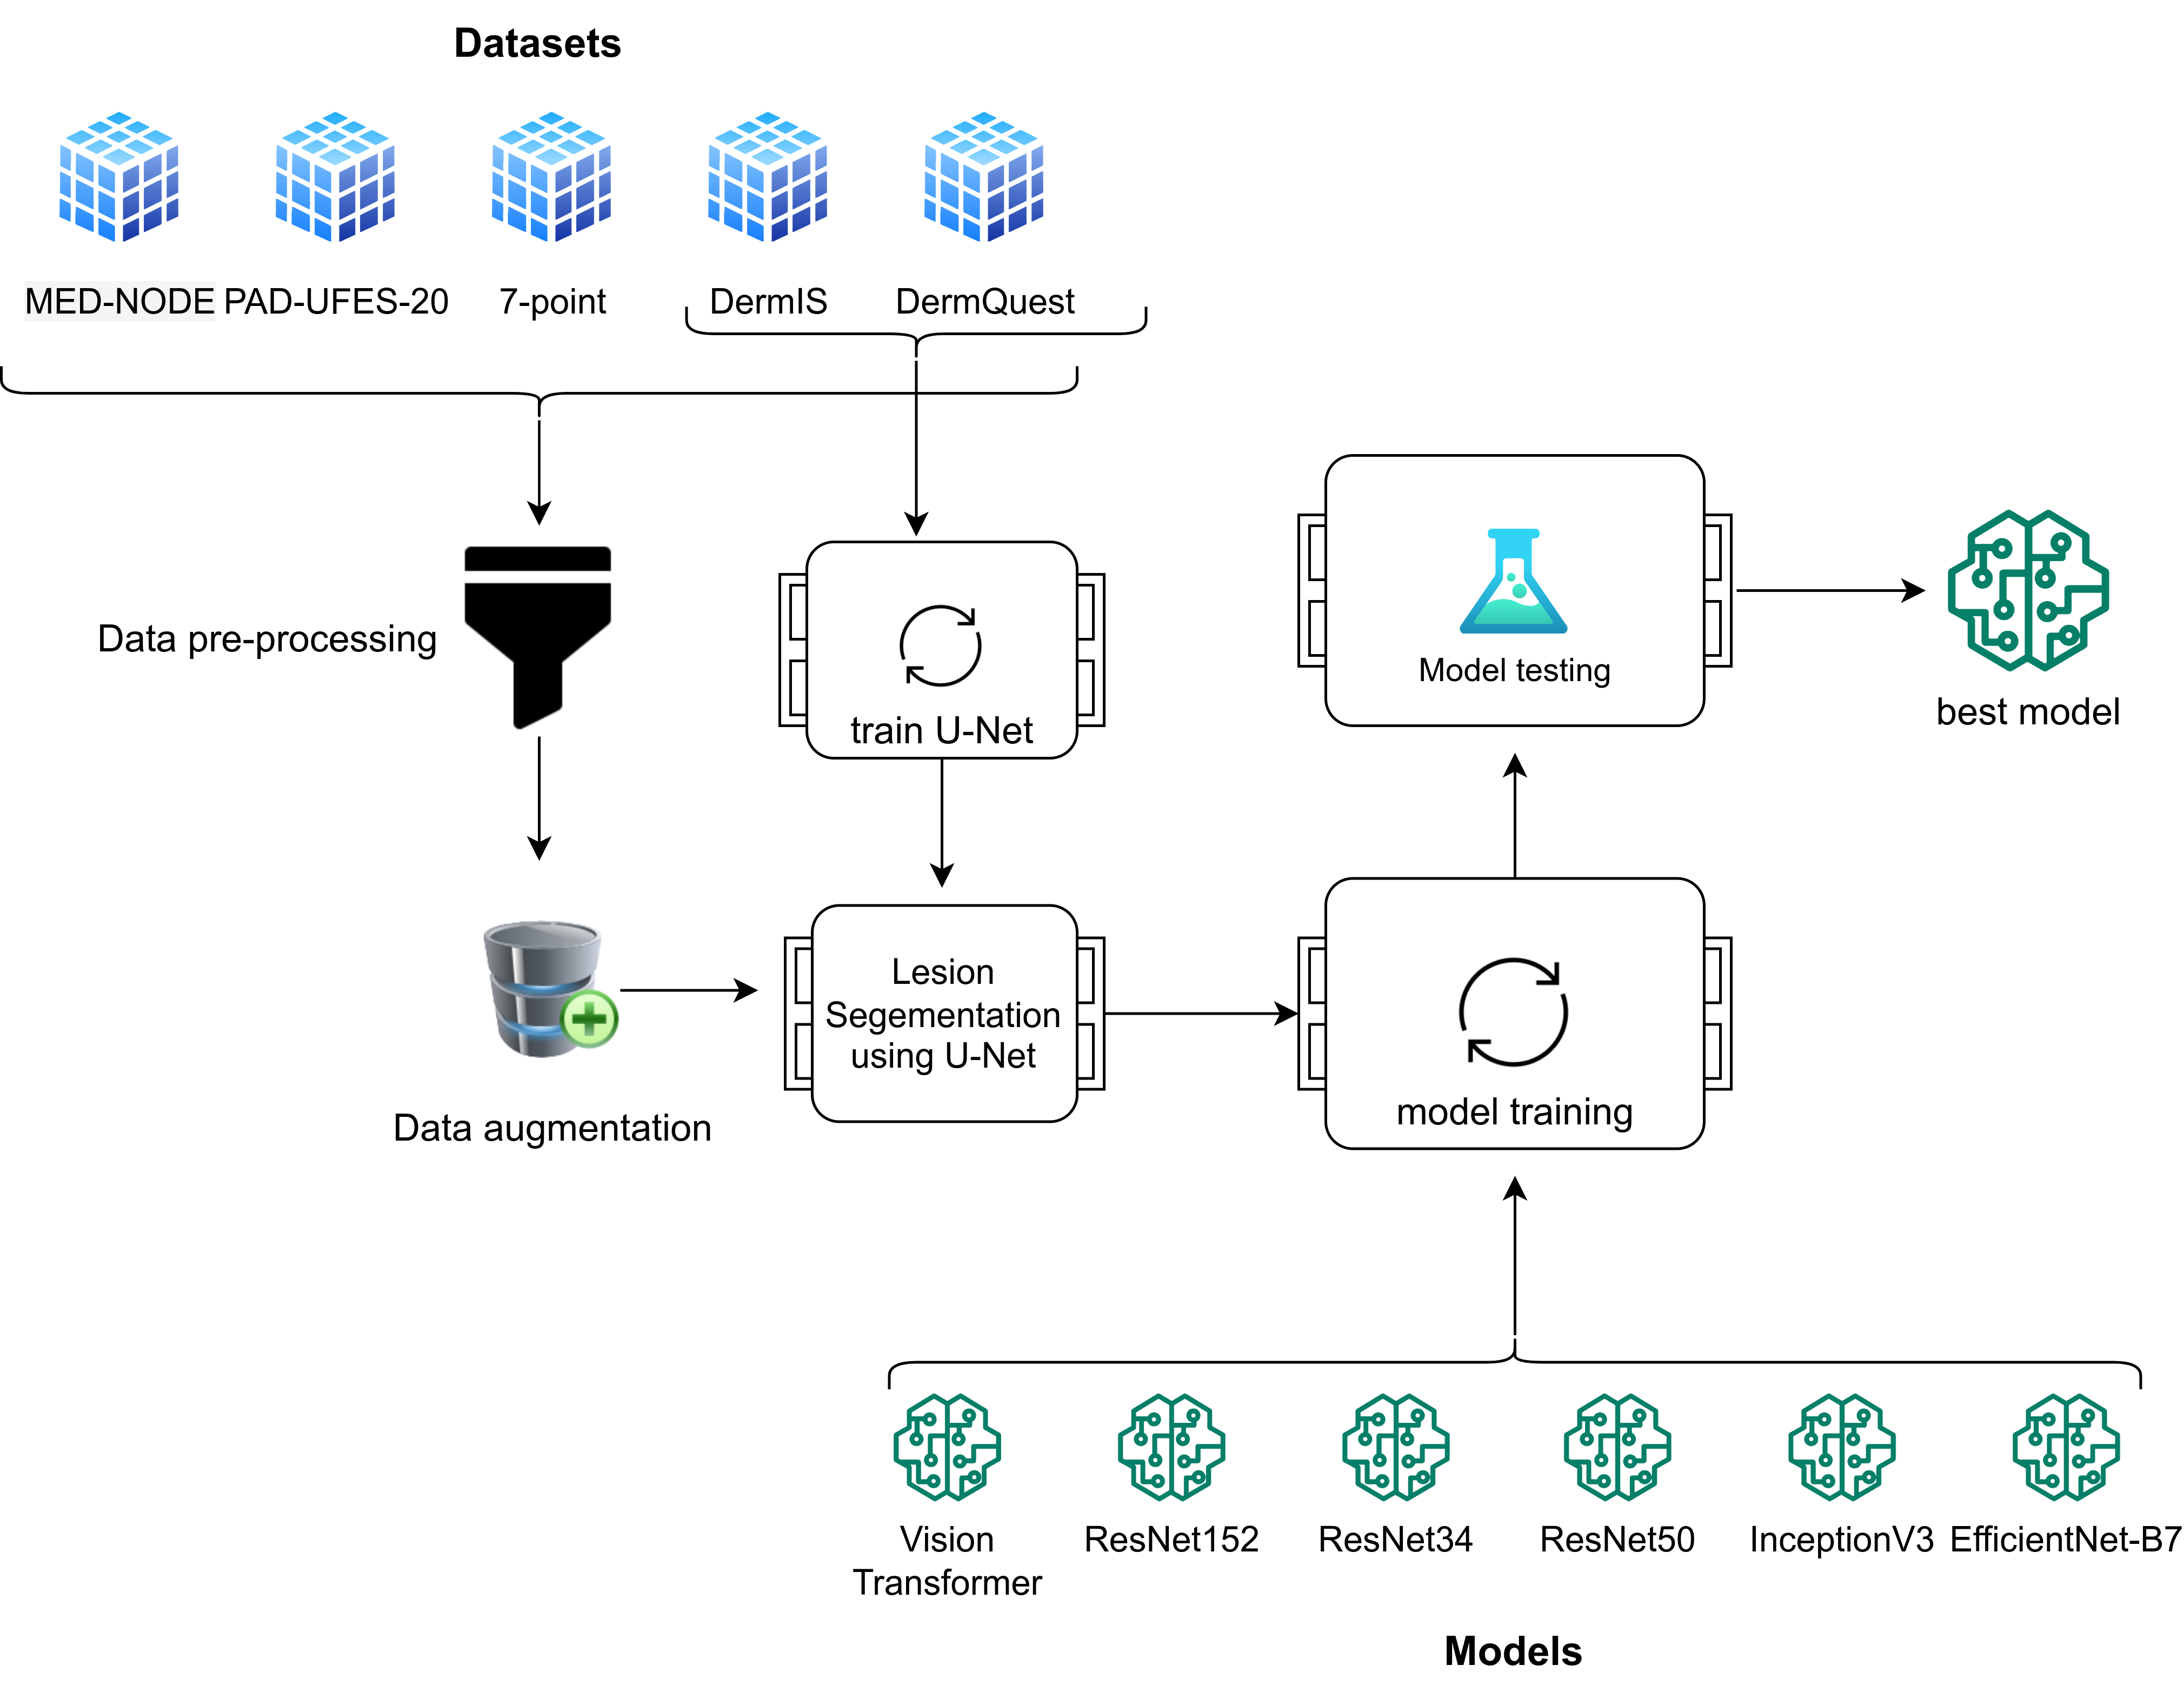
\includegraphics[scale=0.1, fbox]{concept.png}
    \caption{Conceptual framework}
    \label{fig:concept}
\end{figure}
\clearpage
\section{Methodology}
\subsection{Introduction}
This chapter discusses the design paradigm and methodology used in the development of the developed solution. Various analysis and design diagrams used are outlined, deliverables for the developed solution are discussed and finally, the tools and techniques used in development are presented.

The design paradigm used is the Object-Oriented Analysis and Design (OOAD) paradigm. OOAD is a design approach that simplifies real-world systems by using the concept of objects and their interaction to model systems in software development~\citep{nerson1992applying}. OOAD was more suited to the development of the solution since the design of the system is greatly simplified by conceptualization using objects, and OOAD is flexible as it allowed the developed solution to be iterated on to produce an optimal version of the solution.
\subsection{Methodology}
The methodology applied was the incremental development methodology. According to \cite{sommerville2011software}, the incremental development methodology involves the development of an initial implementation of a solution followed by the evolution of that implementation, also called an increment, through a series of iterations till an optimal satisfaction of the requirements is obtained. Figure \ref{fig:methodology} below shows a diagrammatic depiction of the incremental development methodology.

The incremental development methodology was suited to the development of the developed solution since the nature of the solution demands iteration. Deep learning involves training models over numerous epochs and tuning hyperparameters hence requiring a lot of iterations. The incremental development methodology involves three major activities which are discussed below namely, specification, development and validation. These activities were repeated with each iteration.
\subsubsection{Requirements Specification}
The requirements specification phase involves the collection of the requirements for the system and their analysis. In this phase, requirements for the developed solution were defined through document analysis of existing technological solutions. With every subsequent iteration, this phase was repeated.
\begin{figure}[h]
    \centering
    \setlength{\fboxsep}{8pt}
    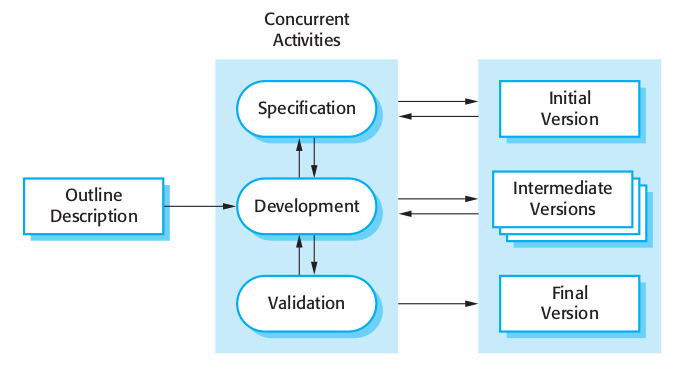
\includegraphics[scale=0.5, fbox]{sommerville.png}
    \caption{Depiction of the incremental methodology from \citep{sommerville2011software}}
    \label{fig:methodology}
\end{figure}
\subsubsection{Development}
The development phase involves the designing and implementation of a system guided by the requirements specification. For each iteration, during this phase, the developed solution was designed and built as per the requirements specified in the previous phase.
\subsubsection{Validation}
The validation phase involves ascertaining that the implementation of the development phase does indeed conform to the requirements specification guiding its development. The ascertainment was done through testing. Each increment was validated during this phase.
\subsection{Analysis Diagrams}
\subsubsection{Use Case Diagram}
A use case diagram is a diagram that shows the high-level functions of a system and how various actors interact with those functions. The use case diagram was used to analyse the actors and functions of the developed system.
\subsubsection{Entity Relationship Diagram}
An Entity Relationship Diagram (ERD) is a diagram that depicts the high-level entities in a system and the relationship among them. The ERD diagram was used to analyse the entities involved in the developed solution, their relationships and cardinality.
\subsubsection{Sequence Diagram}
A sequence diagram is an object-oriented system modelling diagram that shows the sequential interaction of objects within a system. The sequence diagram was used to analyse how the objects in the developed solution were to interact to successfully segment and classify skin
lesion images.
\subsubsection{System Sequence Diagram}
A system sequence diagram is an object-oriented system modelling diagram that shows the sequential interaction of external actors with a system. The sequence diagram was used to analyse how the external actors were to interact with the developed solution to successfully segment and classify skin lesion images.
\subsubsection{Activity Diagram}
An activity diagram is a Unified Modelling Language (UML) diagram that depicts the flow of activities of events of a system for a given use case or multiple use cases. The activity diagram was used to analyse the flow of activities and events during the segmentation and classification of a skin lesion image.
\subsubsection{Class Diagram}
A class diagram is a UML diagram that models a system by depicting the system's classes, class attributes, class operations and the relationship between the objects defined by the classes. The class diagram was used to analyse how the entities of the developed system would be mapped into classes and the relationship between the classes.
\subsection{Design Diagrams}
\subsubsection{Database Schema}
A database schema diagram depicts the structure of tables which correspond to entities in a system and the relationship between the tables. The database schema diagram was used to design a suitable database design for the developed system.
\subsubsection{Wireframes}
Wireframes are line drawings which depict how the user interface of a system will be structured. Wireframes were used to design the user interface and simulate the user experience of the developed system.
\subsubsection{System Architecture Diagram}
A system architecture diagram is a diagram that depicts the interaction of the top-level independent functional units of a system. The system architecture was used to design the functional units of the developed solution and to profile their interaction.
\subsection{Deliverables}
\subsubsection{Research Proposal}
A research proposal is a formal document that outlines what research is about by stating the title, discussing background information of the area of research, stating objectives, justification, scope and limitations, reviewing the literature on the area of research and discussing the methodology for the research project. The research proposal justified the research and guided the implementation of the developed solution.
\subsubsection{Project Documentation}
The project documentation is a formal document that outlines what the project is about by stating the title, discussing background information of the area of research, stating objectives, justification, scope and limitations, reviewing the literature on the area of research, discussing the methodology for the research project, implementation and testing of the developed system and ends with conclusions, recommendations and points out future works.
\subsubsection{Deep Learning Model}
A deep learning model refers to a deep neural network (a network with many layers of perceptrons) whose weights have been trained to perform a classification or regression task. The deep learning model was the core of the developed solution as it was responsible for the segmentation and classification of skin lesion images. The model was deployed on a server and exposed as an Application Programming Interface (API).
\subsubsection{Mobile App User Interface}
A mobile app was developed to provide a user interface through which users can use the deep learning model to classify skin lesion images. The app worked by accessing the camera of a mobile device to take a photo of a skin lesion image and then uploading the photo to the API hosting the deep learning model. Once the deep learning model determined the verdict, the mobile app notified the user of the results of the classification.
\subsection{Tools and Techniques}
\subsubsection{Python}
Python was used as the programming language in the implementation of the developed solution. This was because the majority of the machine learning and data science community used Python as the programming language of choice~\citep{raschka2015python}. Hence many indispensable tools for machine learning and deep learning supported python more than other languages.
\subsubsection{PyTorch}
PyTorch is a machine-learning framework maintained by Facebook. PyTorch was suited to this project compared to other machine learning frameworks since according to \cite{he2019mlframeworks} it was gaining more popularity in research being published meaning it was deemed as better suited for research. PyTorch also provided more ease of development compared to other machine learning frameworks since it is more "pythonic" and uses a more object-oriented style~\citep{simmons2019comparison}.
\subsubsection{Google Colaboratory}
Google Colaboratory, also known as Google Colab, was used to execute the Python code that implemented the developed solution. This is because Google Colab is a free Software as a Service(SaaS) application by Google that offers free Graphics Processing Units (GPU) and hence was used to efficiently train the machine learning models of the developed solution.
\subsubsection{Expo}
Expo was used to develop the mobile application. Expo is a framework built on top of React Native which exposes an API for building cross-platform mobile applications using purely JavaScript while abstracting the complexity of having to write native code on Xcode or Android Studio. React Native, released by Facebook is a framework that allows building cross-platform mobile applications using React syntax. Expo was used since it allowed the development of a cross-platform mobile application.
\subsubsection{Data Augmentation}
According to \cite{perez2021convolutional}, data augmentation is a technique of expanding the size of a dataset by applying several random transformations to original images. Since non-dermoscopic datasets were small there was a need to augment them to reduce overfitting. \cite{perez2021convolutional}, in a comparative study showed that all the models used in the study substantially performed better with data augmentation.
\subsubsection{Transfer Learning}
According to \cite{perez2021convolutional}, transfer learning is a technique of reusing already trained models from a source task which has a lot of data for a different but related task. \cite{esteva2017dermatologist}, \cite{HAN20181529} and \cite{perez2021ensemble} all use transfer learning in the form of pre-trained deep learning models showing a performance improvement. Therefore transfer learning was applied in this study to increase model performance.
% \subsubsection{K-Fold Cross-Validation}
% According to \cite{refaeilzadeh2009cross}, k-fold cross-validation is a technique of evaluating model performance by dividing the training dataset into k folds such that for each iteration k-1 folds are used for training while one fold is held out to be used for validation. K-fold cross-validation was used for validation since the dataset used was relatively small having 711 images.
\clearpage
\section{System Analysis and Design}
\subsection{Introduction}
This chapter discusses how the system exposing the developed model was analysed and designed. Functional and non-functional system requirements are discussed and OOAD paradigm system analysis and design diagrams are presented and elaborated upon.
\subsection{System Requirements}
The system requirements for the developed system are as follows.
\subsubsection{Functional Requirements}
Functional requirements refer to the set of operations that a system must be able to provide~\citep{glinz2007non}. The functional requirements of the developed system include:
\begin{enumerate}[i.]
    \item Authentication Module --- This module provided registration and login functionality to users. The authentication module was needed so that users can keep records of their transactions with the system.
    \item Image Capture and Upload Module --- This module was implemented in a mobile application to enable users to take a picture of a skin lesion and upload it to a server hosting the developed model for inference.
    \item Lesion Inference Module --- This module consisted of the developed model which would take a lesion image as input and perform inference by segmentation followed by classification of whether the lesion is malignant melanoma or a benign mole. This module also included a user interface in the mobile app that will relay the results of the inference to the user.
\end{enumerate}
\subsubsection{Non-Functional Requirements}
Non-functional requirements refer to the set of characteristics, attributes or constraints of a system which are desirable but not necessary for the functioning of a system~\citep{glinz2007non}. The non-functional requirements for the developed system include:
\begin{enumerate}[i.]
    \item System Security --- Given that the system dealt with medical data which tends to be sensitive, maximum privacy needed to be ensured. Passwords were hashed during the onboarding of users to guard against password breaches. All communication between the server and the client app was restricted to being over HTTPS only, hence ensuring that all data was encrypted in transit.
    \item System Performance --- The system was built to minimise response time to requests as much as possible, thus ensuring a delightful user experience.
\end{enumerate}
\subsection{System Analysis Diagrams}
\subsubsection{Use Case Diagram}
Figure \ref{fig:use-case} shows the use-case diagram for the developed system. The actors are the user and a Machine Learning (ML) model. The user can register with the system, login into the system, take a photo of a lesion and upload an image of a lesion upon which the lesion image is normalized in preparation for lesion inference. The ML Model can perform lesion classification on an uploaded image. Lesion classification includes lesion segmentation.
\begin{figure}[h]
    \centering
    \setlength{\fboxsep}{8pt}
    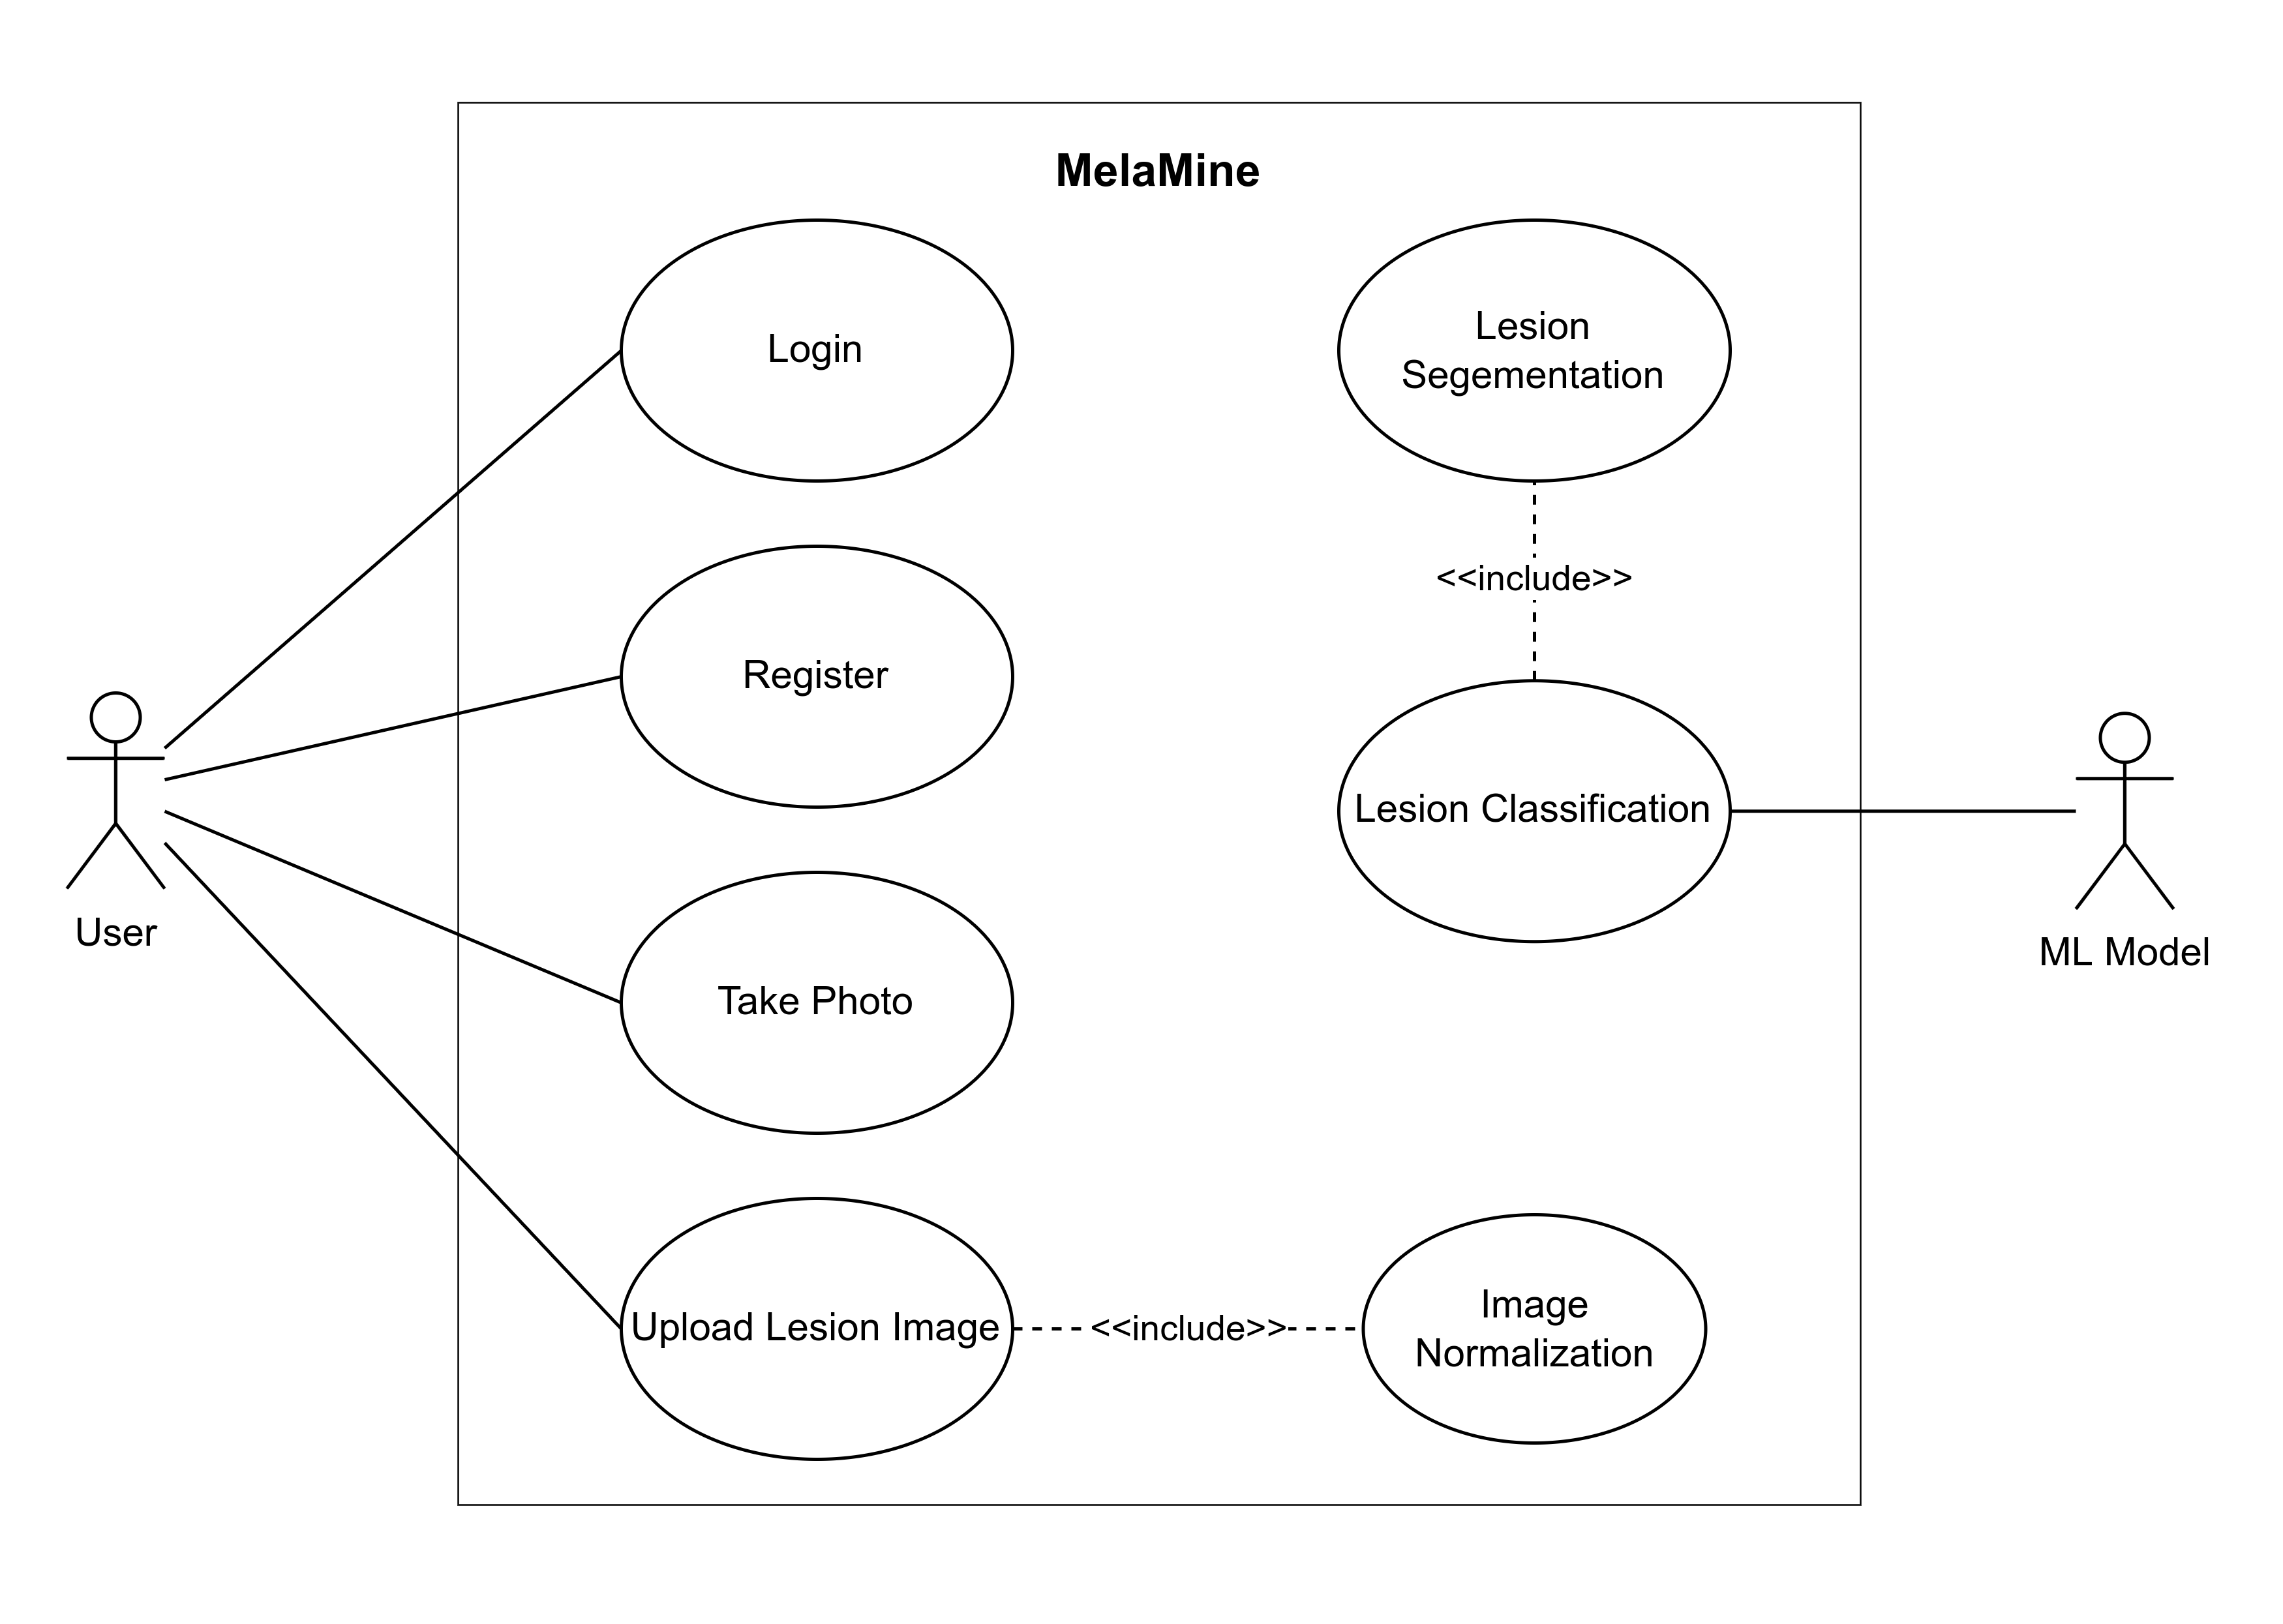
\includegraphics[scale=0.12, fbox]{use-case.png}
    \caption{Use case diagram}
    \label{fig:use-case}
\end{figure}
\subsubsection{Entity Relationship Diagram}
Figure \ref{fig:erd} shows the ERD for the developed system. The developed system consists of three top-level entities namely, the user, a lesion and an ML model. The user has the unique identifier `userId', an email and a password. A lesion has the following attributes: the unique identifier `lesionId', an image file of the lesion, a malignancy truth value and a timestamp. A user bears zero or more lesions and the ML model classifies zero or more lesions as malignant or benign.
\begin{figure}[h]
    \centering
    \setlength{\fboxsep}{8pt}
    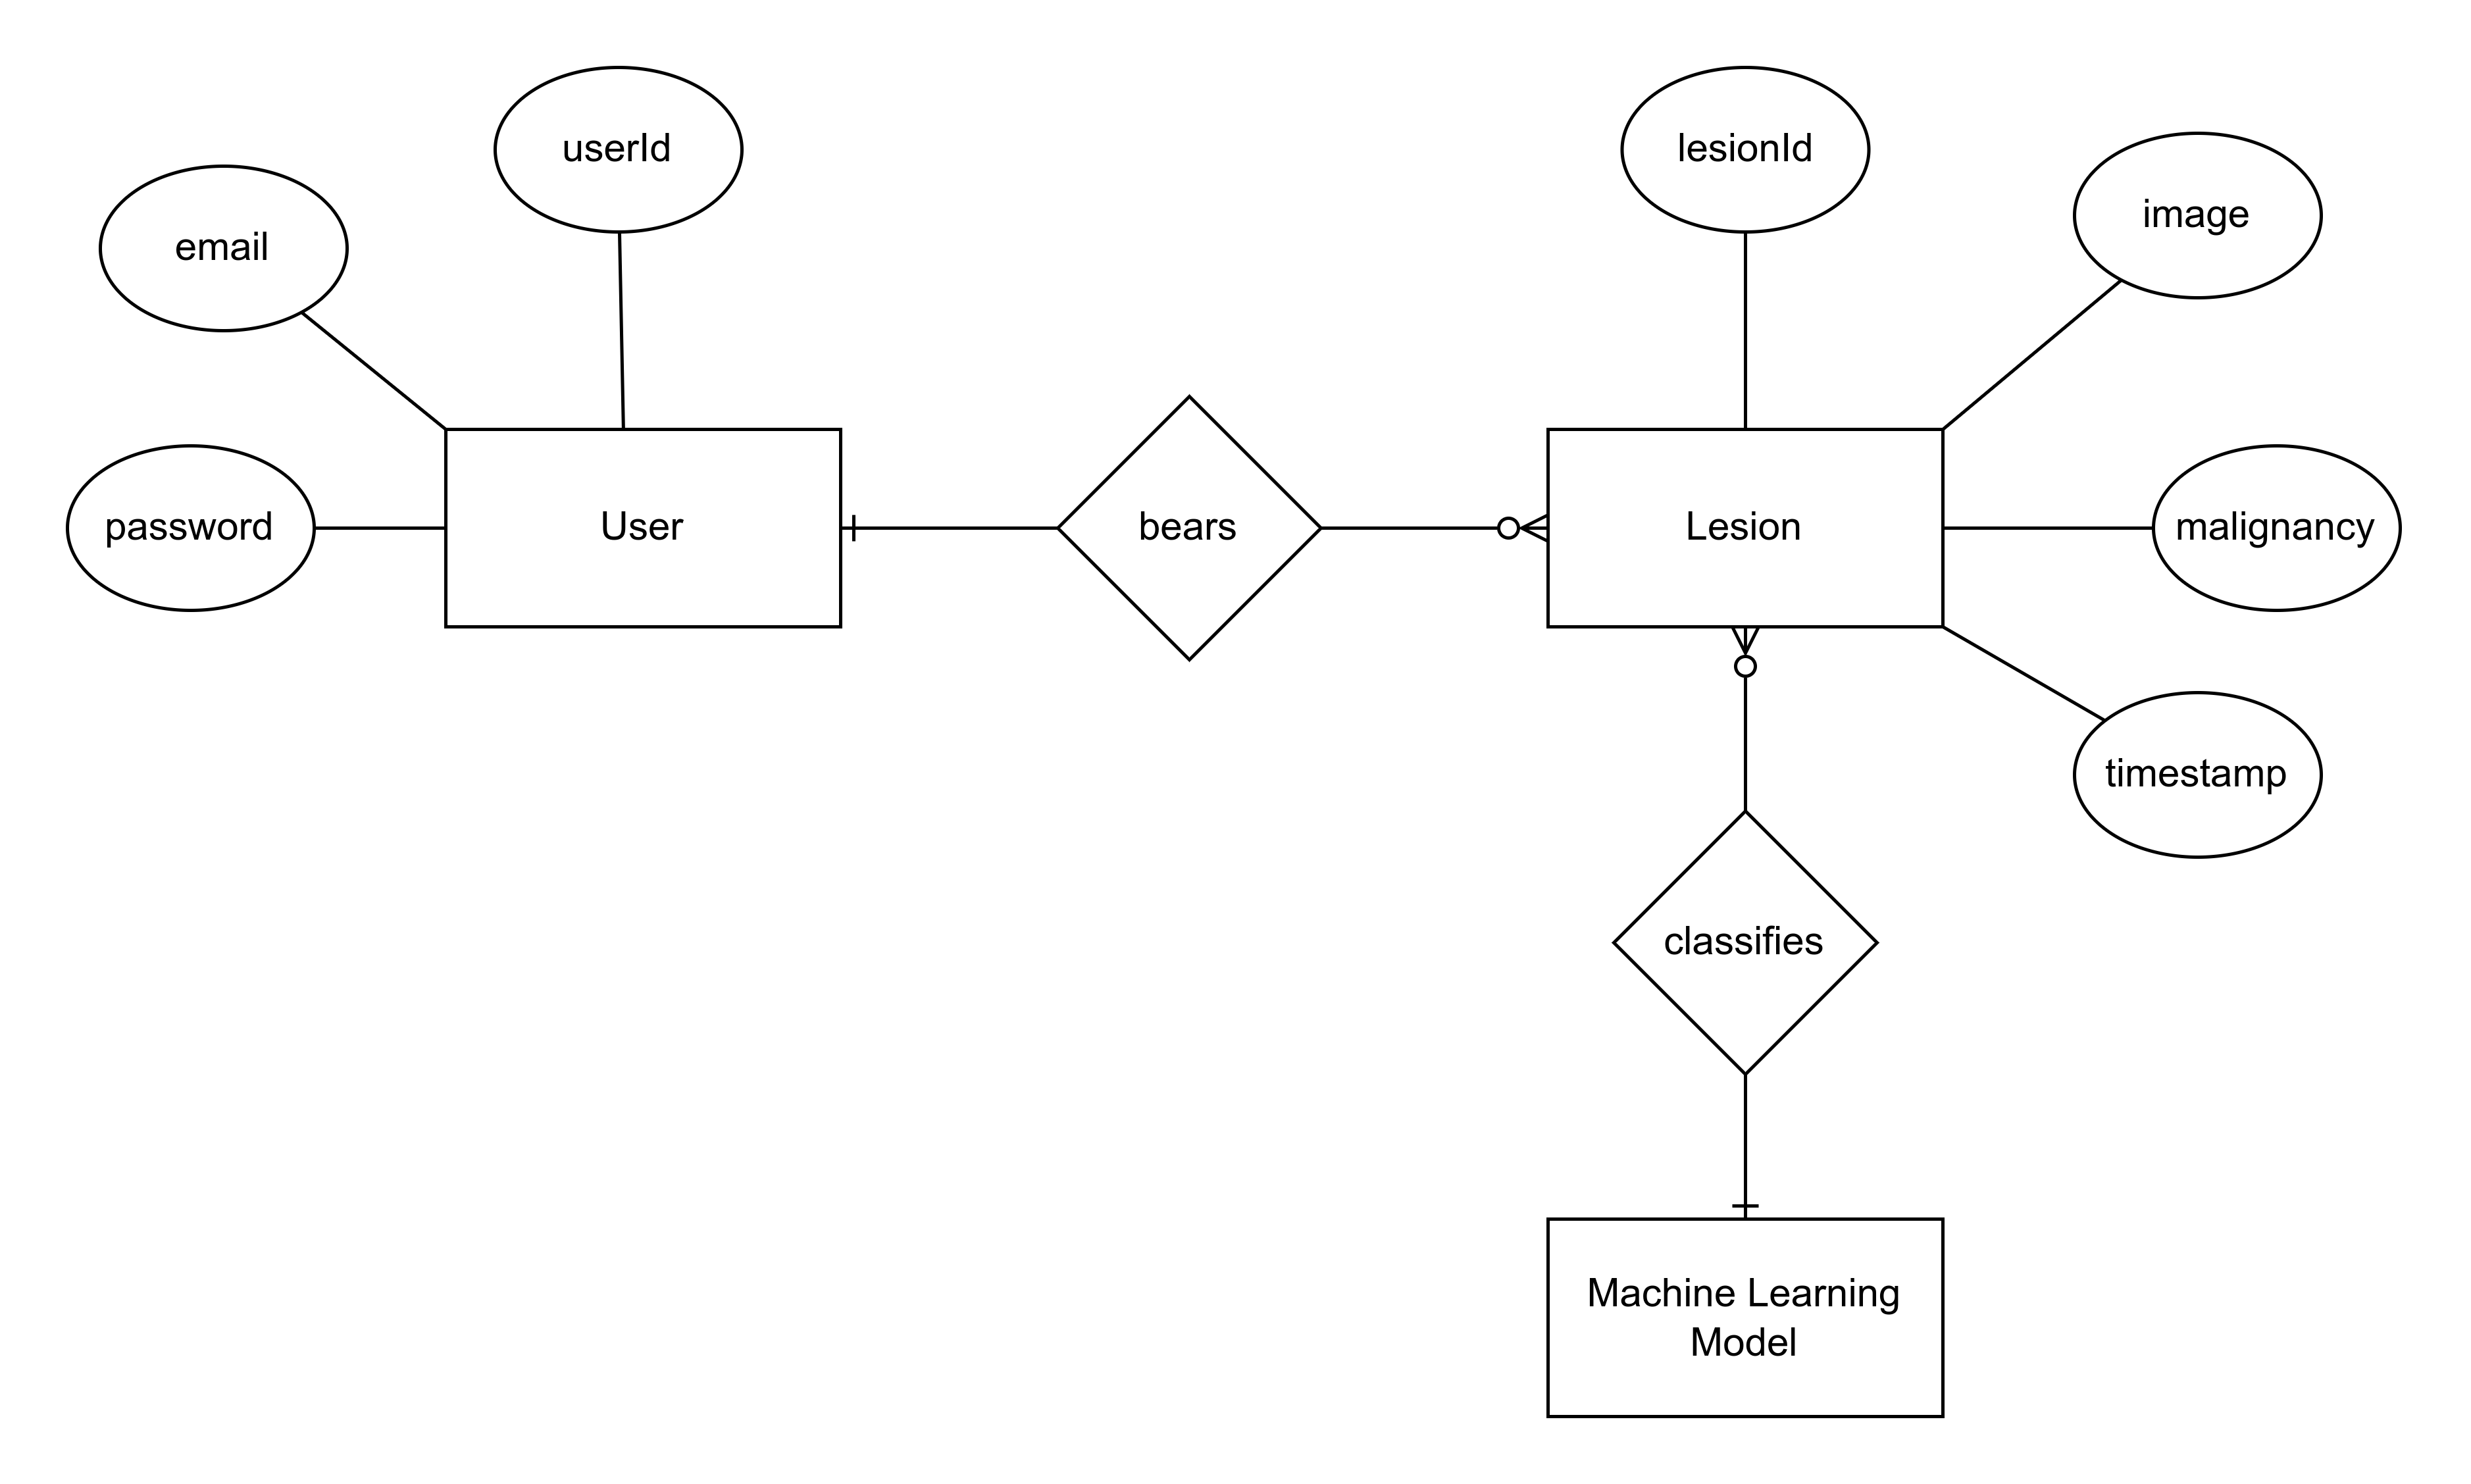
\includegraphics[scale=0.115, fbox]{erd.png}
    \caption{Entity Relationship Diagram}
    \label{fig:erd}
\end{figure}
\subsubsection{Sequence Diagram}
Figure \ref{fig:sequence-diagram} shows the sequence diagram for the developed system. It depicts how the instances of User, Lesion and Model classes interact during lesion inference. The user object invokes the lesion object's setLesionImage method hence setting the image of the lesion to be classified. Subsequently, the user object invokes the isMalignant method of the lesion object and awaits for an inference result.

The lesion object subsequently invokes normalizeImage method to normalize the lesion image and calls the model object's getInference method. Consequently, the model object invokes its segment method and uses its classify method to classify the lesion and returns the inference result to the lesion object which in turn returns the inference result to the user object.
\begin{figure}[h]
    \centering
    \setlength{\fboxsep}{8pt}
    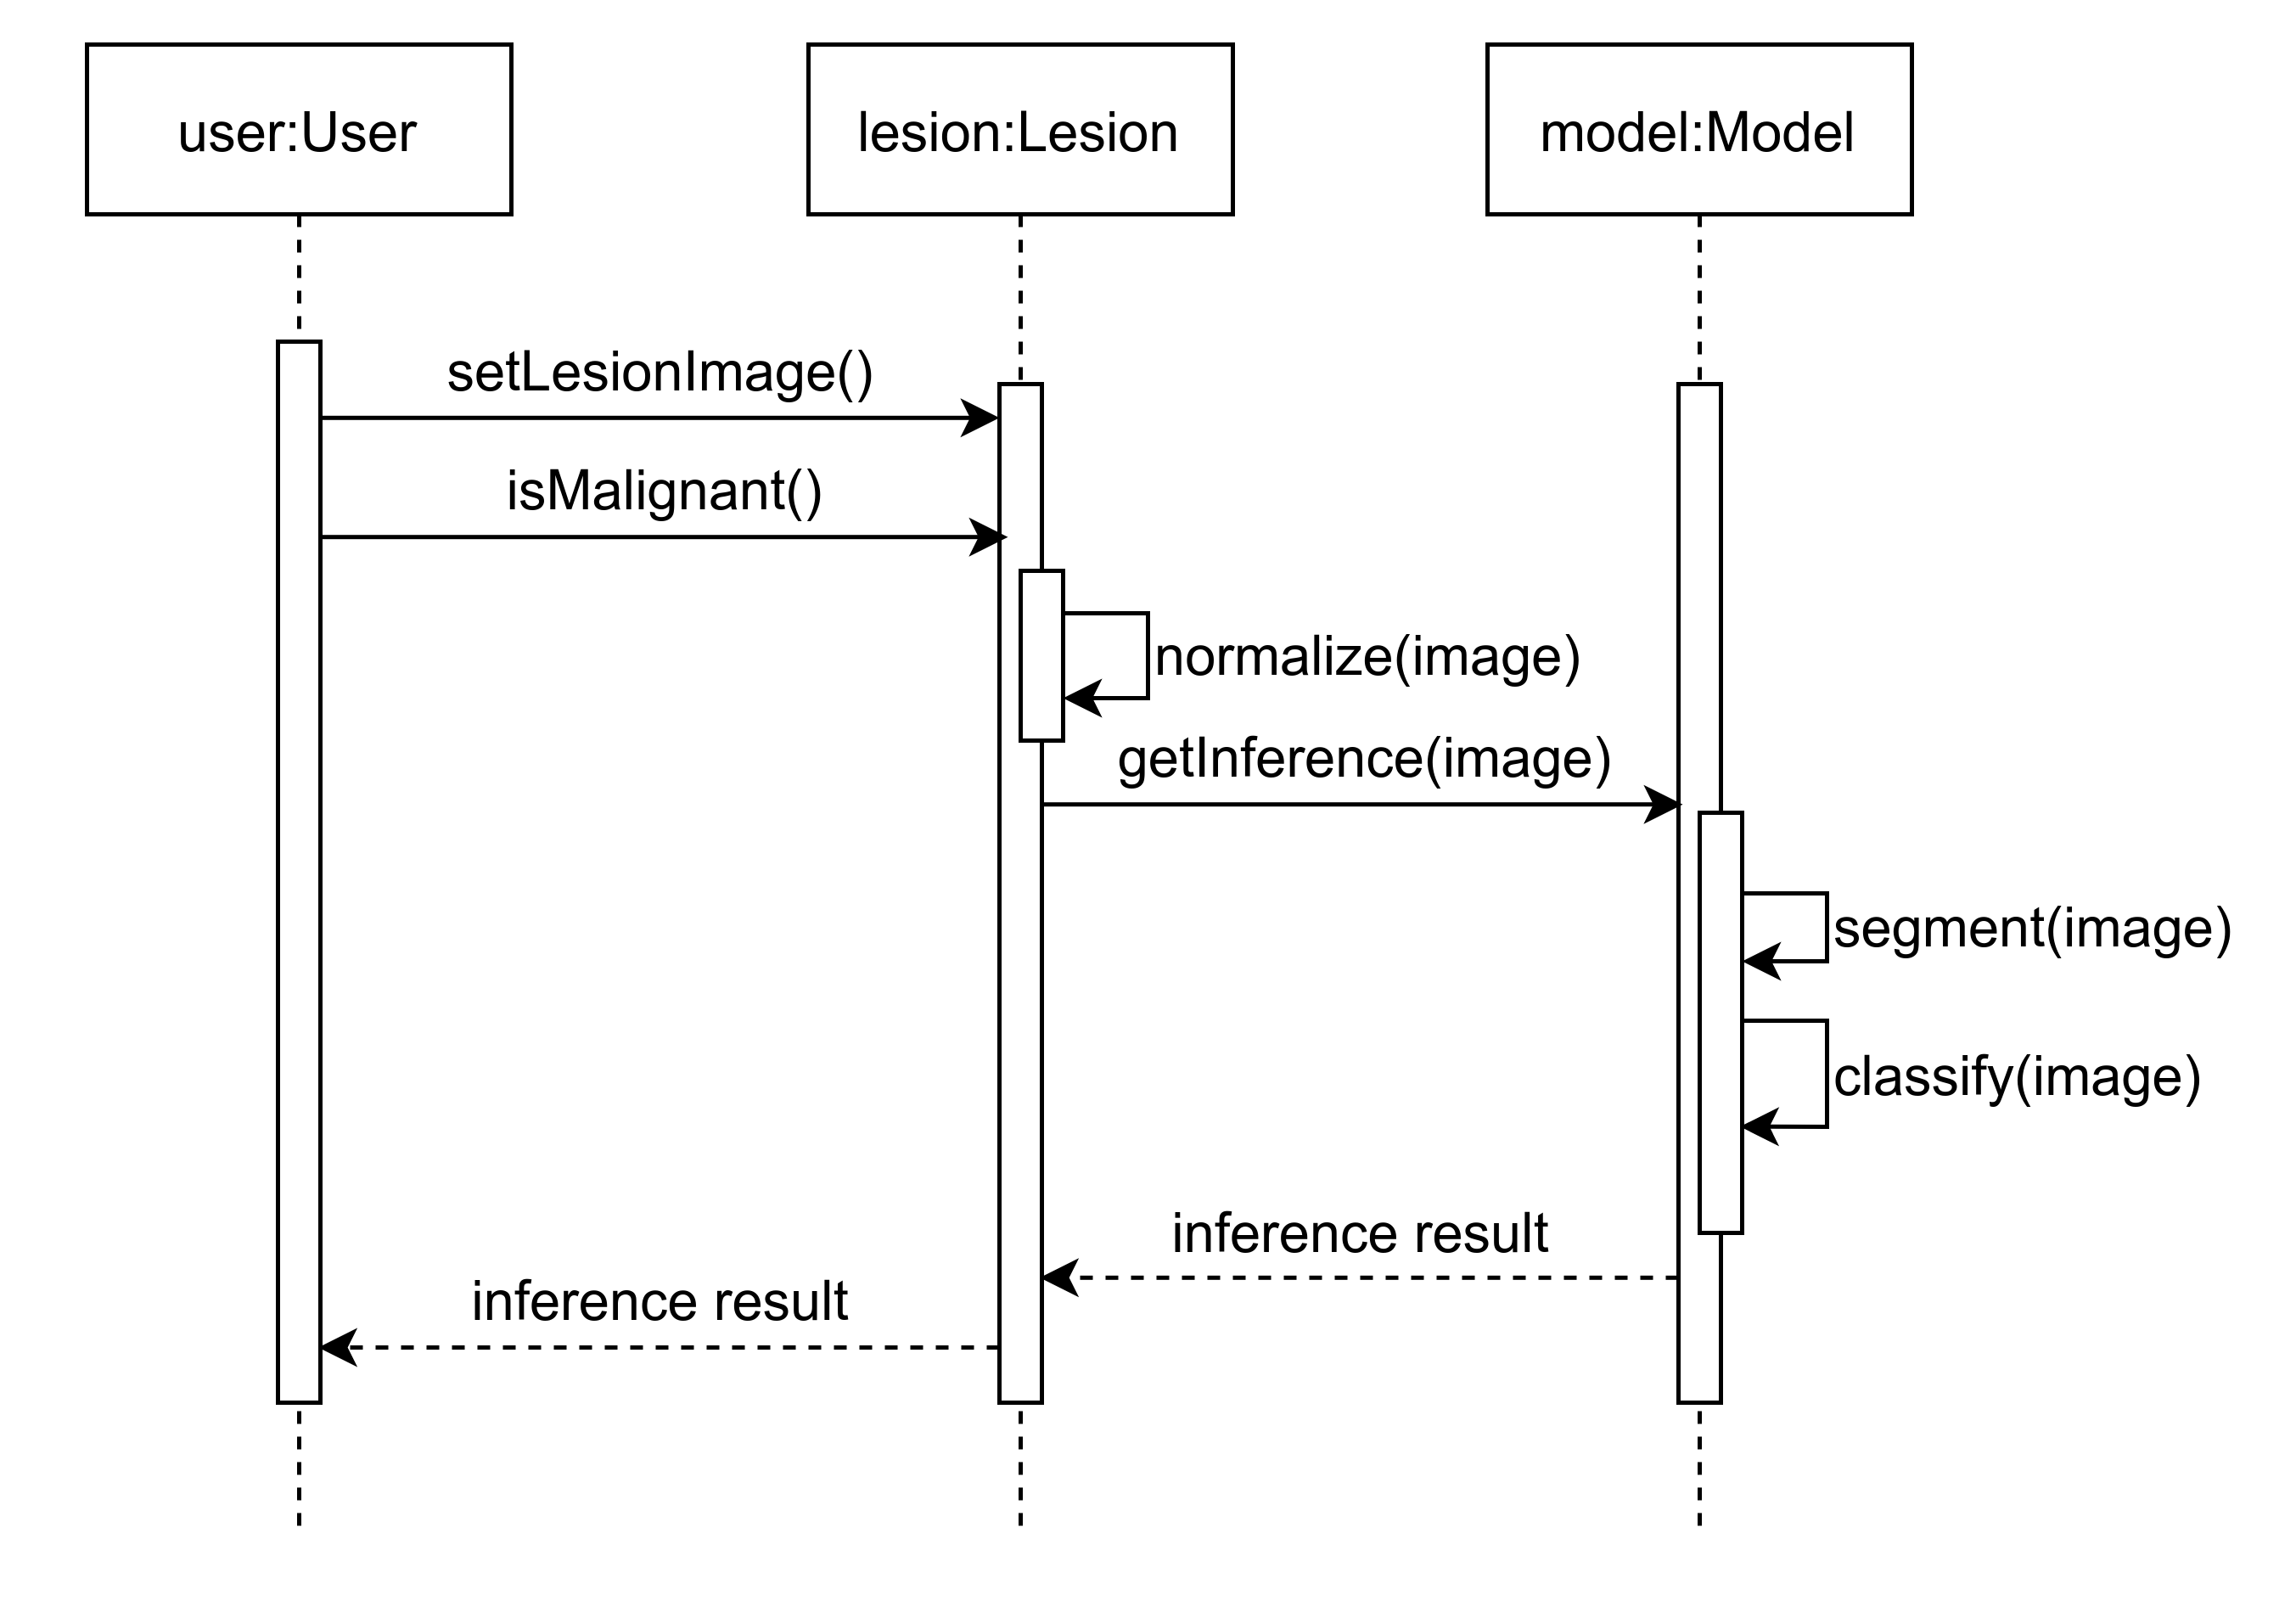
\includegraphics[scale=0.15, fbox]{sequence-diagram.png}
    \caption{Sequence diagram}
    \label{fig:sequence-diagram}
\end{figure}
\subsubsection{System Sequence Diagram}
Figure \ref{fig:sys-sequence-diagram} shows the system sequence diagram for the developed system. The sequence diagram depicts how a user can classify a lesion. The user wishing to log in is authenticated using an email and password combination by making a login request to the web server through the mobile app. If the credentials are correct the login is successful and the user takes a photo of a lesion or selects an existing image. The user, through the mobile app, then uploads the lesion image to the server. The server normalizes the image through resizing, cropping and transformation. The normalized image is then segmented and classified by the ML Model which then passes the result of inference back to the server which in turn relays the inference result back to the user through the mobile app.
\begin{figure}[h]
    \centering
    \setlength{\fboxsep}{8pt}
    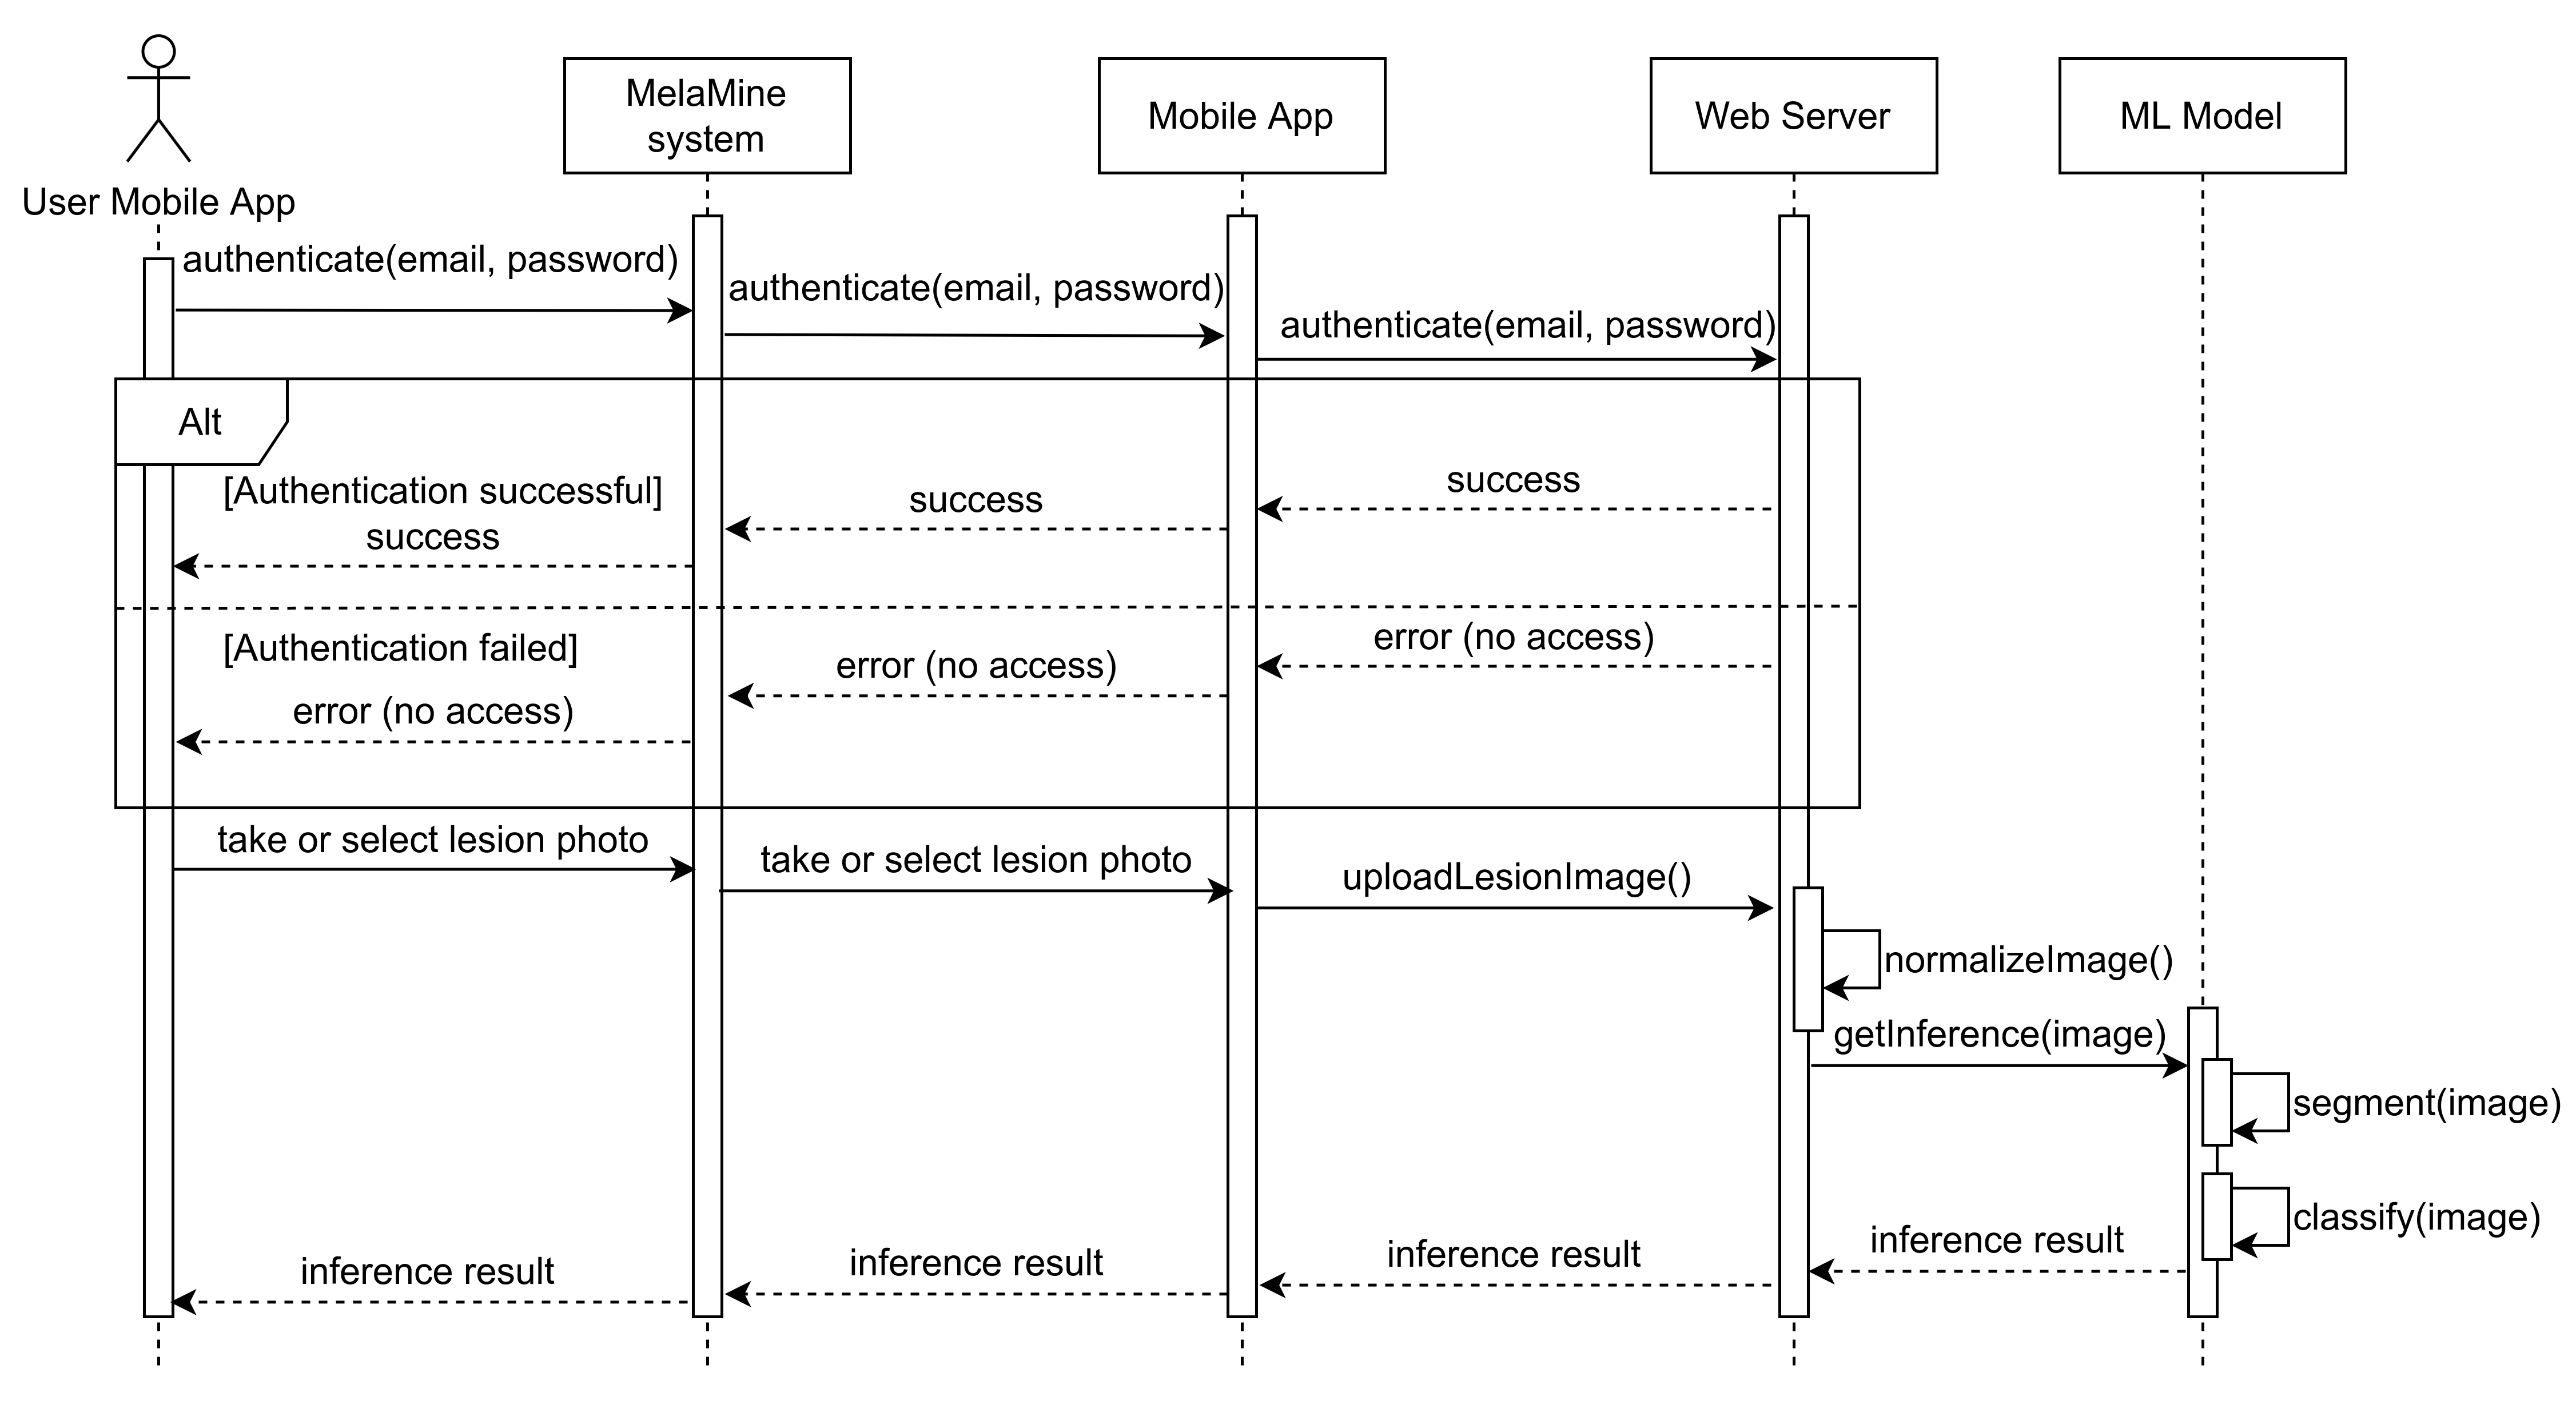
\includegraphics[scale=0.0965, fbox]{sys-sequence-diagram.png}
    \caption{System sequence diagram}
    \label{fig:sys-sequence-diagram}
\end{figure}
\subsubsection{Activity Diagram}
Figure \ref{fig:activity-diagram} shows the activity diagram for the developed system. The activity diagram describes the activity by which a user can obtain inference for a skin lesion. There are four actors namely, the user, the mobile app, the web server and the ML model.
\begin{figure}[h]
    \centering
    \setlength{\fboxsep}{8pt}
    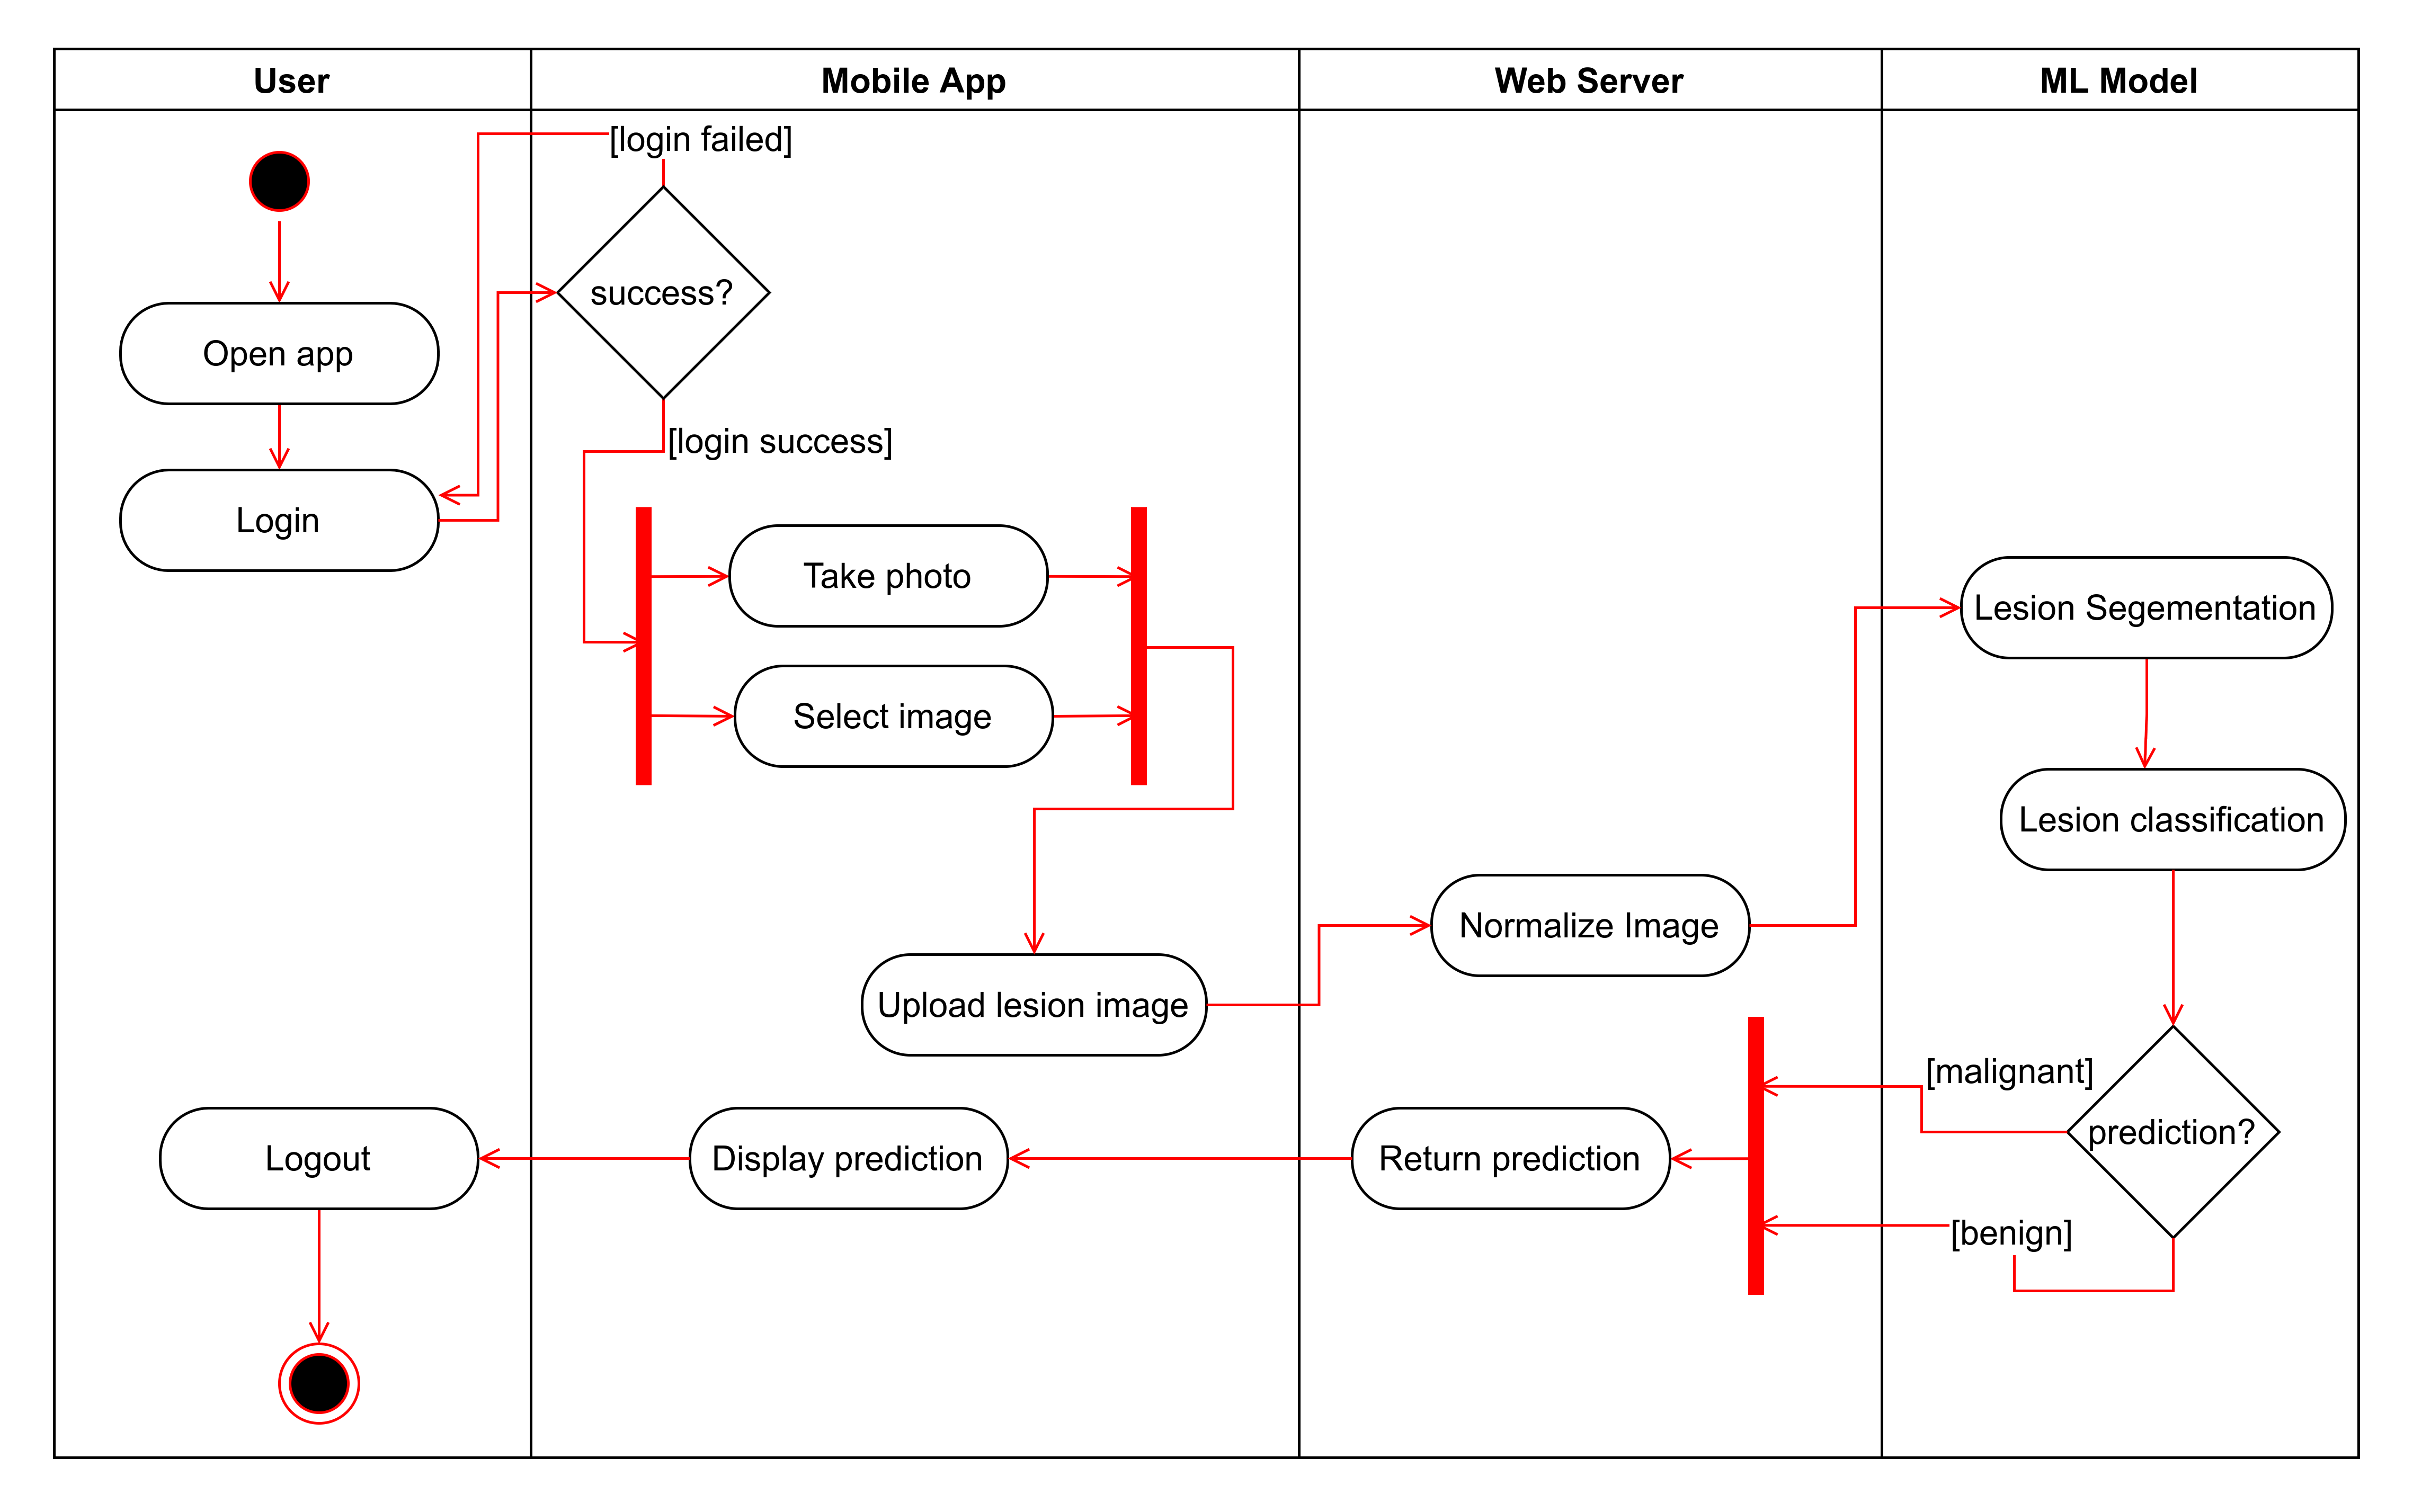
\includegraphics[scale=0.096, fbox]{activity-diagram.png}
    \caption{Activity diagram}
    \label{fig:activity-diagram}
\end{figure}

At the start of the activity, the user opens the mobile application and attempts a login action which succeeds if the user enters a valid username and password combination but fails otherwise. If the login attempt is successful, the user uses the mobile app to either take a photo of a lesion or select an existing image of a lesion. The resulting image is then uploaded to the web server by the mobile app. The web server performs normalization on the uploaded image through resizing, cropping and transformation. The ML model then performs lesion segmentation on the normalized image and subsequently classifies it as either malignant or benign. The results of classification are then relayed back to the web server which returns it to the mobile app which then displays it to the user. The user may then log out.
\subsubsection{Class Diagram}
Figure \ref{fig:class-diagram} shows the class diagram for the developed system. The system has three classes namely: User, Lesion and Model classes. The User class has the userId, email properties and the register and login methods. The userId property uniquely identifies a user. The register method creates a new account for a user. The login method authenticates a user.

\begin{figure}[h]
    \centering
    \setlength{\fboxsep}{8pt}
    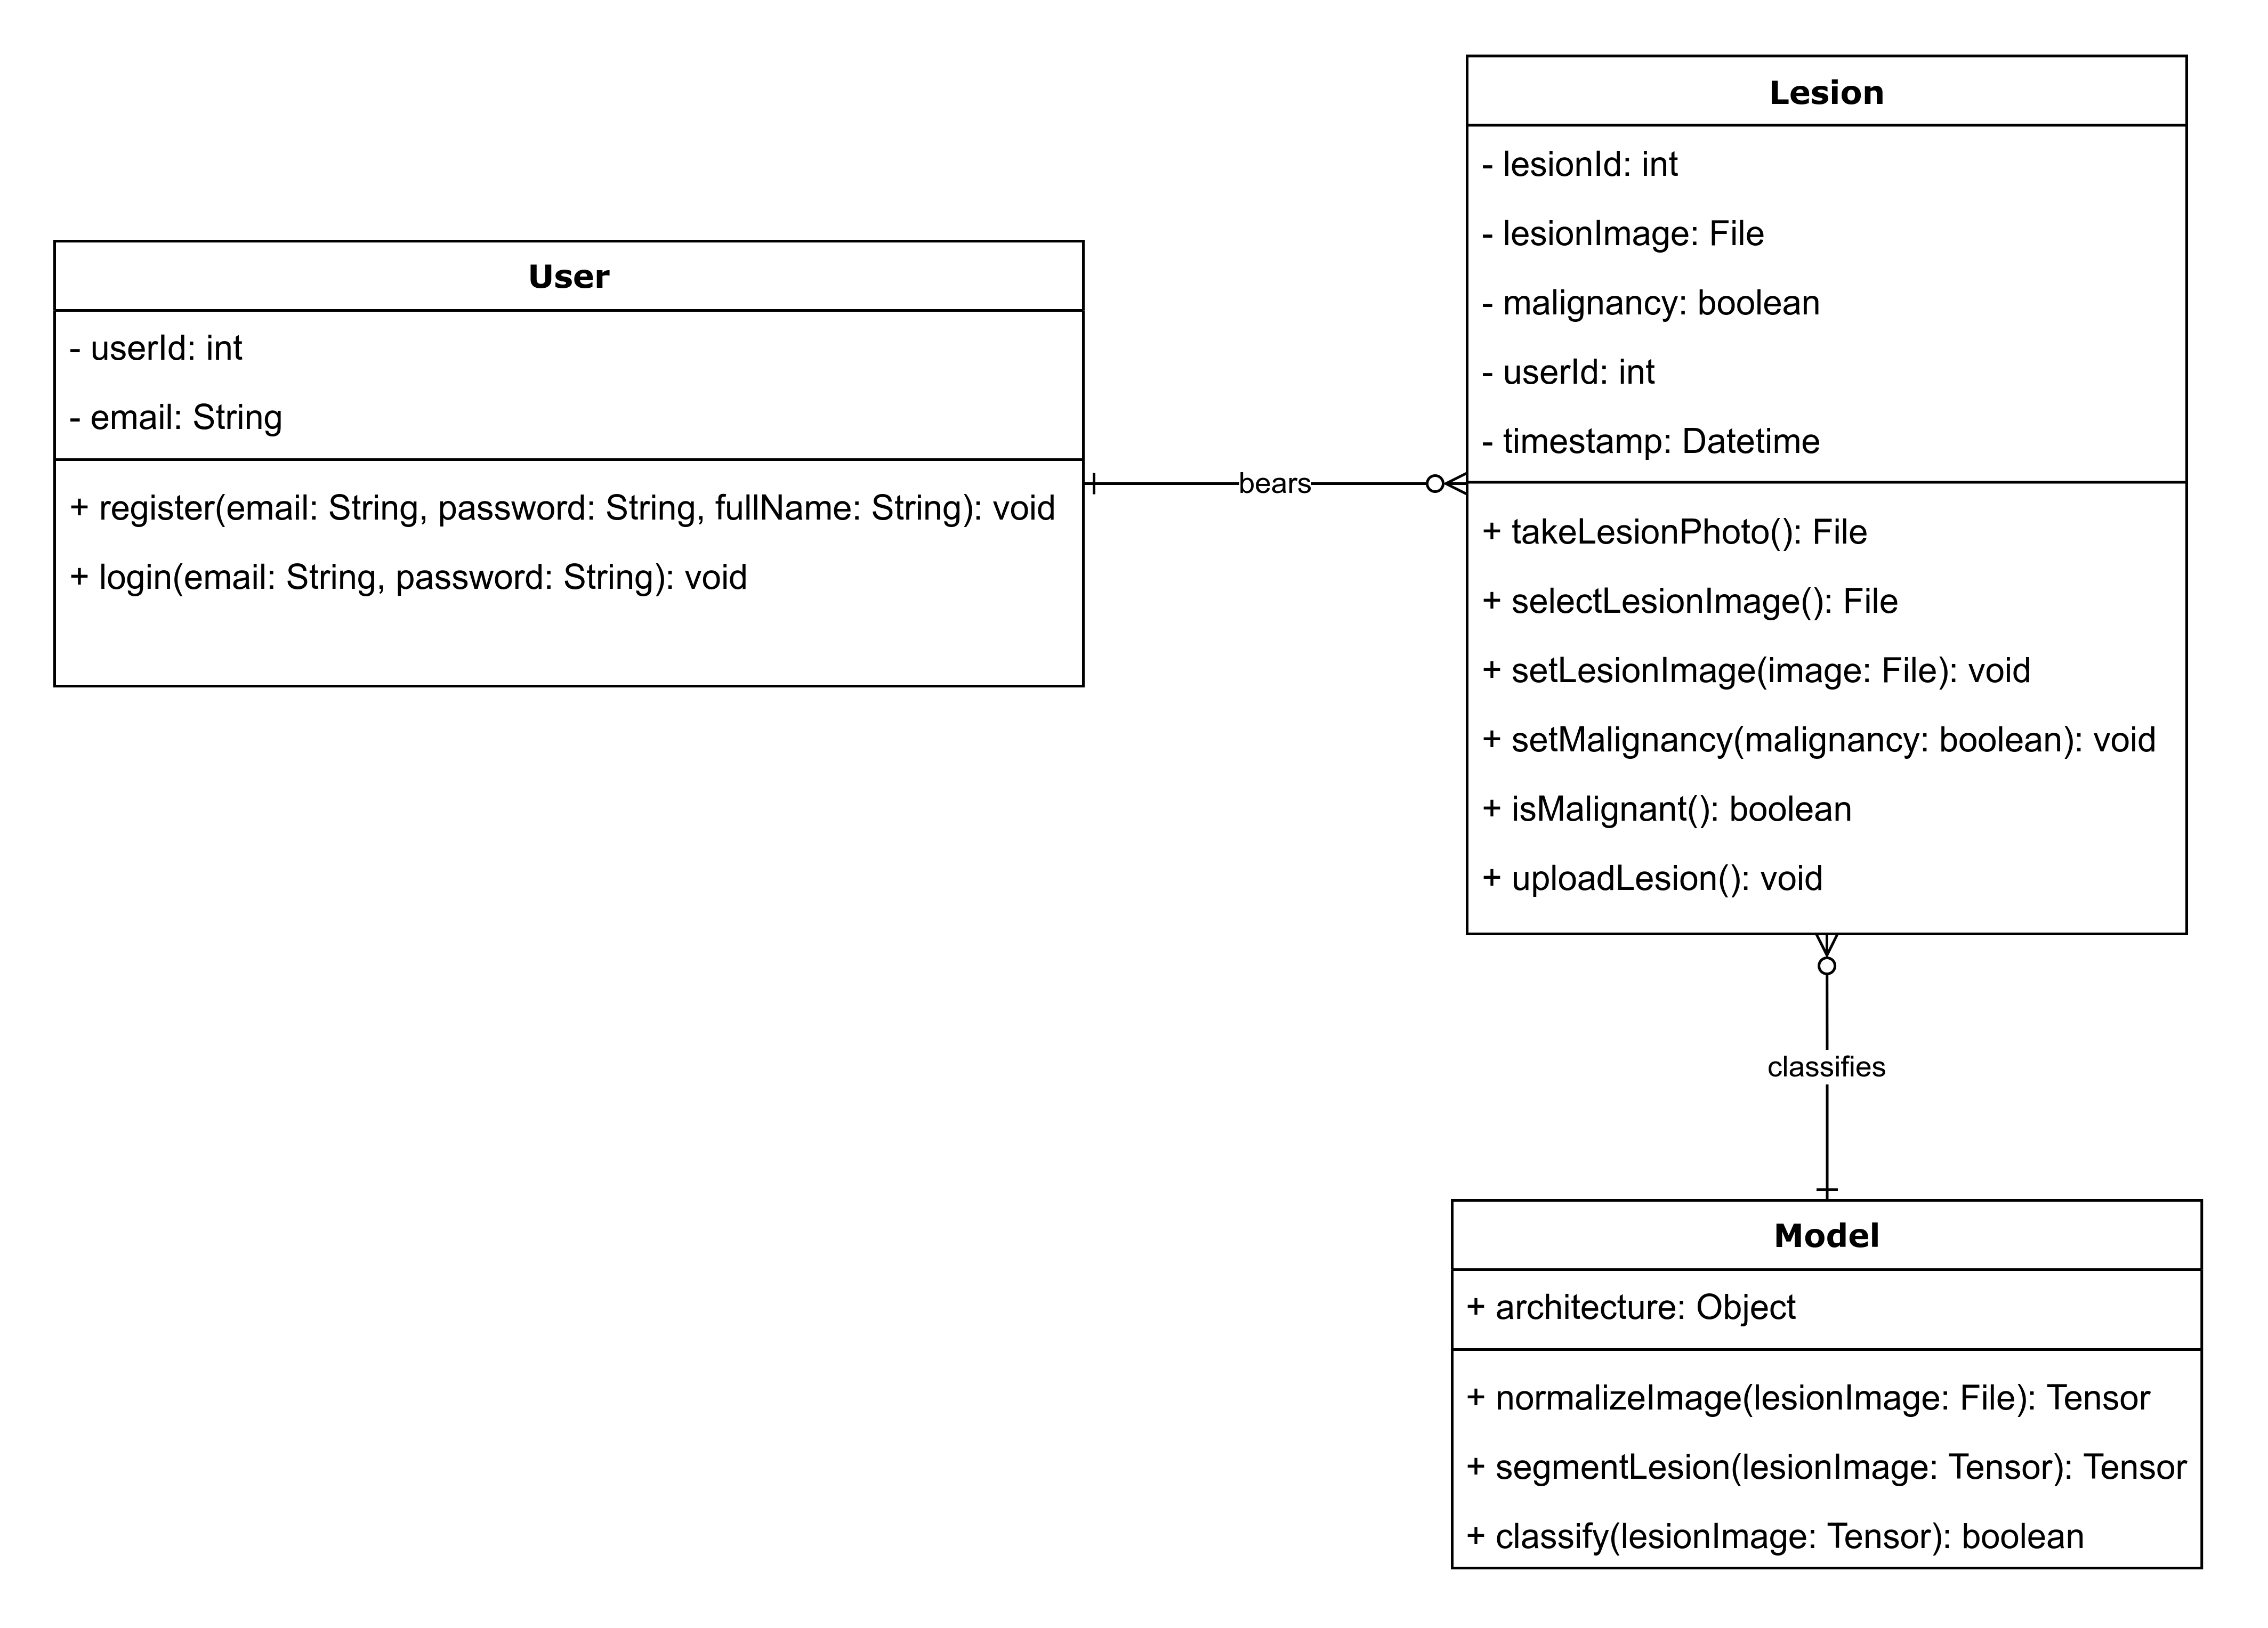
\includegraphics[scale=0.1, fbox]{class-diagram.png}
    \caption{Class diagram}
    \label{fig:class-diagram}
\end{figure}

The Lesion class has lesionId, lesionImage, malignancy, userId, timestamp properties and takeLesionPhoto, selectLesionImage, setLesionImage, setMalignancy, isMalignant, uploadLesion methods. The lesionId property uniquely identifies a lesion, the lesionImage property stores an image file of the lesion, the malignancy property stores a truth value of whether the lesion is malignant or benign and the timestamp property stores the date and time of the creation of a lesion record in the database. The takeLesionPhoto method access the camera on the phone, takes a photo and returns it. The selectLesionImage method allows the user to select an existing lesion image from the file system. The setLesionImage method is used to set the lesionImage property upon capturing of an image or selection from the file system. The isMalignant method uses the uploadLesion method to upload an image of a lesion to the web server requesting for inference on the lesion, waits on the request and upon the resolution of the request returns a truth value of the inference. The setMalignancy method is a mutator for the malignancy property.

The Model class wraps the architecture of the actual ML model. The Model class provides the normalizeImage method which normalizes an uploaded image in preparation for inference through resizing, cropping and transformation and returns a Tensor representation of the image. The segmentLesion method passes a normalized image tensor to the segmentation model which then returns the resulting tensor. The classify method passes a segmented Tensor lesion image to the ML model, obtains inference and returns it.

\subsection{System Design Diagrams}
\subsubsection{Database Schema}
Figure \ref{fig:db-schema} shows the database schema for the developed system. The database consists of two tables namely: User and Lesion tables. The User table has the user\_id, email and password attributes. The user\_id attribute is the primary key and hence uniquely identifies every single user record. The email and password attribute store the user credentials that is, email and hashed password respectively.

The Lesion table has the lesion\_id, user\_id, lesion\_img\_url, lesion\_malignancy and lesion\_timestamp attributes. The lesion\_id is the primary key and hence identifies each lesion record uniquely. The user\_id attribute is a foreign key that creates a relationship with the User table such that any lesion belongs to exactly one user. The lesion\_img\_url attribute store the URL of a lesion's image and the lesion\_malignancy nullable attribute stores the inference result of a lesion using either of the two enum values, 0 for benign and 1 for malignant. The lesion\_timestamp attribute stores the date and time of the creation of a lesion record.

\begin{figure}[h]
    \centering
    \setlength{\fboxsep}{8pt}
    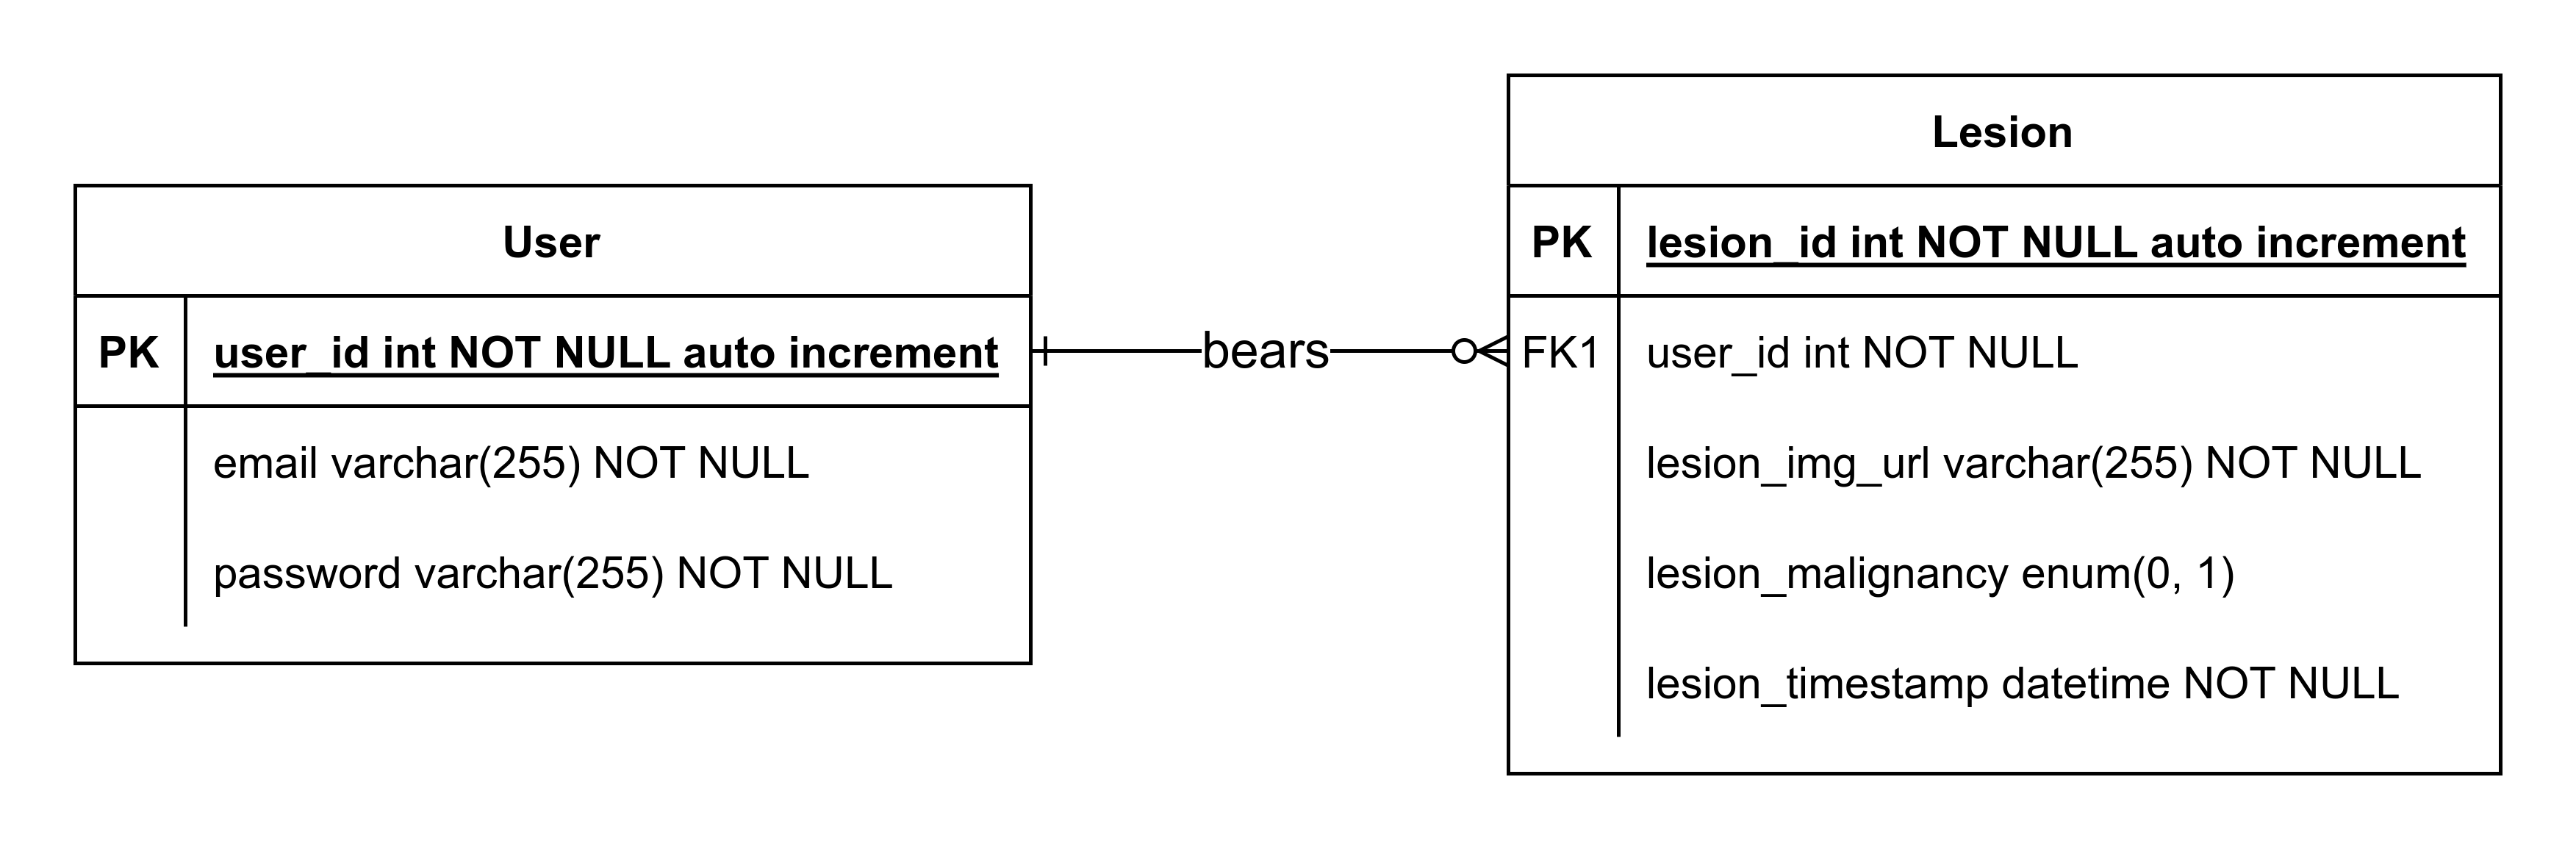
\includegraphics[scale=0.12, fbox]{db-schema.png}
    \caption{Database Schema}
    \label{fig:db-schema}
\end{figure}
\subsubsection{Wireframes}
\paragraph{Authentication Screens}
Figure \ref{fig:login} shows the login screen of the developed system. The user is required to enter the correct email and password combination for successful login. The user may also tap on `Register' in order to create an account. Tapping on `Register' routes the user to the registration screen displayed in Figure \ref{fig:register}.

\begin{figure}[h]
    \centering
    \setlength{\fboxsep}{8pt}
    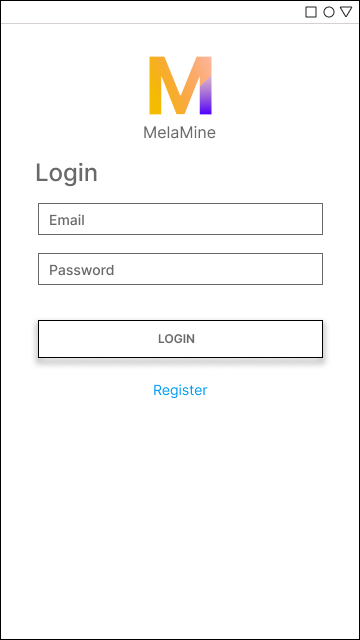
\includegraphics[scale=0.45, fbox]{Login.png}
    \caption{Login screen}
    \label{fig:login}
\end{figure}

On the registration screen, the user is required to enter an email, a new password and its confirmation. The registration is successful if the email address has not been taken and if both the password and its confirmation do match.
\begin{figure}[h]
    \centering
    \setlength{\fboxsep}{8pt}
    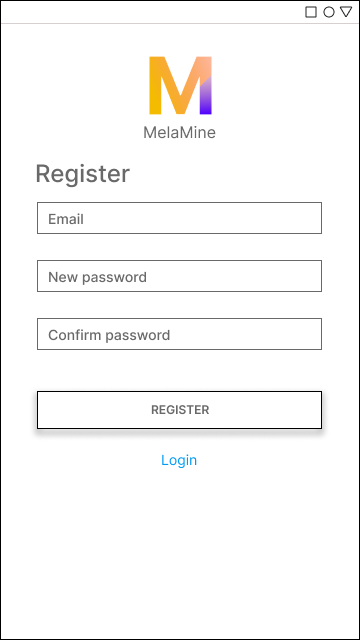
\includegraphics[scale=0.45, fbox]{Register.png}
    \caption{Registration screen}
    \label{fig:register}
\end{figure}
\paragraph{Core Functionality Screens}
Upon successful login, the user is routed to the home screen of the mobile application displayed in Figure \ref{fig:home}. Tapping on the icon at the top-right of the home screen with an arrow going out of an open rectangle, allows the user to log out.

The user may tap on the hamburger icon shown in Figure \ref{fig:home}, upon which the user is routed to the screen in Figure \ref{fig:past_predictions} where a list of predictions made on lesions in the past is displayed. The predictions are sorted by date in descending order. Selecting any of the listed predictions shows the user the image of the lesion and the prediction made on the image as in either Figure \ref{fig:prediction-1} or Figure \ref{fig:prediction-2}.
\begin{figure}[h]
    \centering
    \setlength{\fboxsep}{8pt}
    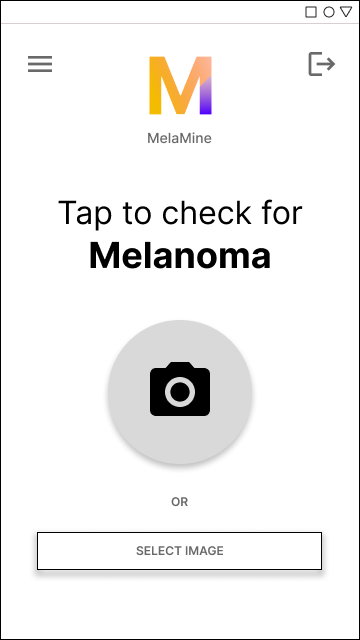
\includegraphics[scale=0.45, fbox]{Home.png}
    \caption{Home screen}
    \label{fig:home}
\end{figure}

On the home screen, the user can tap on the big round button with a camera icon in order to take a photo of a lesion. Alternatively, the user can tap on `SELECT IMAGE' to select an image from the file system instead. If the user selects the camera icon button they are routed to the screen shown in Figure \ref{fig:capture-select} where a live stream for the currently active camera is displayed waiting for the user to take a photo.

Upon taking a photo or selecting an image from the file system the user is routed to the image upload screen shown in Figure \ref{fig:upload}. The user can avoid uploading the currently displayed image by tapping on the `X' button. Otherwise, the user can upload the image for inference by tapping the button with the ``send" icon upon which the user is presented with the screen shown in Figure \ref{fig:waiting} where the user is instructed to wait as the image is uploaded and subsequently undergoing inferencing.

Once inference results have been returned by the server the user is routed to the screen in Figure \ref{fig:prediction-1} if the prediction is positive, that is, the lesion has been predicted as likely to be malignant melanoma. Conversely, if the prediction is negative, that is, the lesion has been predicted as unlikely to be melanoma, the user is routed to the screen in Figure \ref{fig:prediction-2}.
\begin{figure}[h]
    \centering
    \setlength{\fboxsep}{8pt}
    
\includegraphics[scale=0.45, fbox]{CaptureSelect.png}
    \caption{Image capture screen}
    \label{fig:capture-select}
\end{figure}

\begin{figure}[h]
    \centering
    \setlength{\fboxsep}{8pt}
    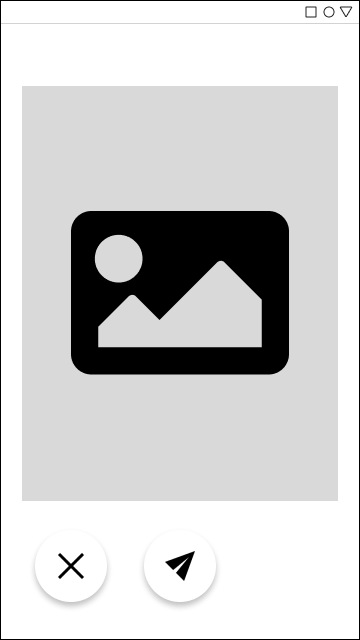
\includegraphics[scale=0.45, fbox]{Upload.png}
    \caption{Image upload screen}
    \label{fig:upload}
\end{figure}

\begin{figure}[h]
    \centering
    \setlength{\fboxsep}{8pt}
    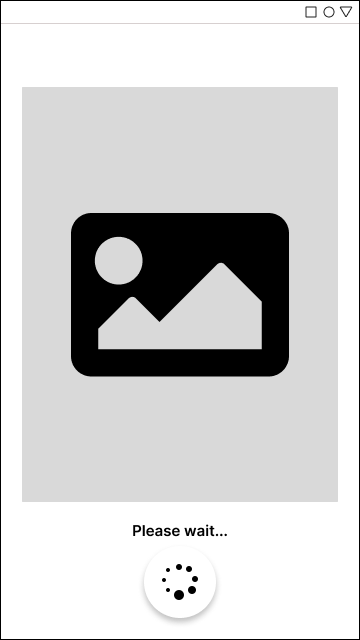
\includegraphics[scale=0.45, fbox]{Waiting.png}
    \caption{Waiting-for-prediction screen}
    \label{fig:waiting}
\end{figure}

\begin{figure}[h]
    \centering
    \setlength{\fboxsep}{8pt}
    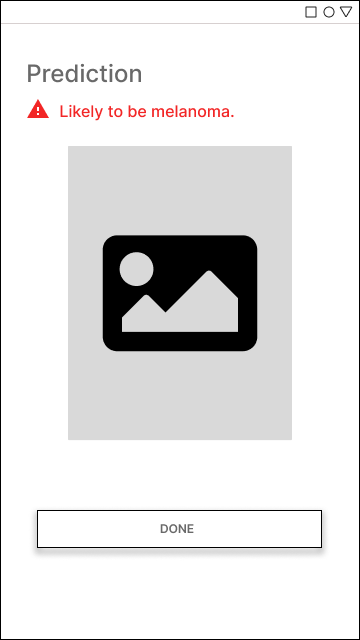
\includegraphics[scale=0.45, fbox]{Prediction-1.png}
    \caption{Positive prediction display screen}
    \label{fig:prediction-1}
\end{figure}

\begin{figure}[h]
    \centering
    \setlength{\fboxsep}{8pt}
    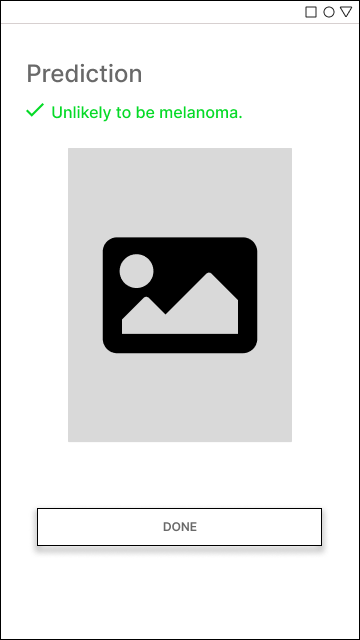
\includegraphics[scale=0.45, fbox]{Prediction-2.png}
    \caption{Negative prediction display screen}
    \label{fig:prediction-2}
\end{figure}

\begin{figure}[h]
    \centering
    \setlength{\fboxsep}{8pt}
    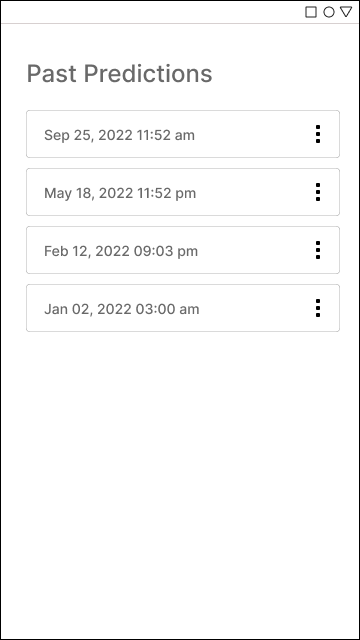
\includegraphics[scale=0.45, fbox]{Predictions.png}
    \caption{Past predictions display screen}
    \label{fig:past_predictions}
\end{figure}
\clearpage
\subsubsection{System Architecture}
Figure \ref{fig:arch-diagram} shows the system architecture diagram for the developed system. The developed system consists of a thin client React Native mobile app, a Flask web server hosting a PyTorch environment where the ML model operates from and a MySQL database. The mobile app allows the user to capture an image or select an image from the file system and upload it to the Flask web server for inference. The Flask web server passes the uploaded image to the ML model and obtains inference results which it then relays back to the mobile app. The Flask web server stores user data and prediction history in the SQL server and mediates data retrieval from the database by the mobile app.
\begin{figure}[h]
    \centering
    \setlength{\fboxsep}{8pt}
    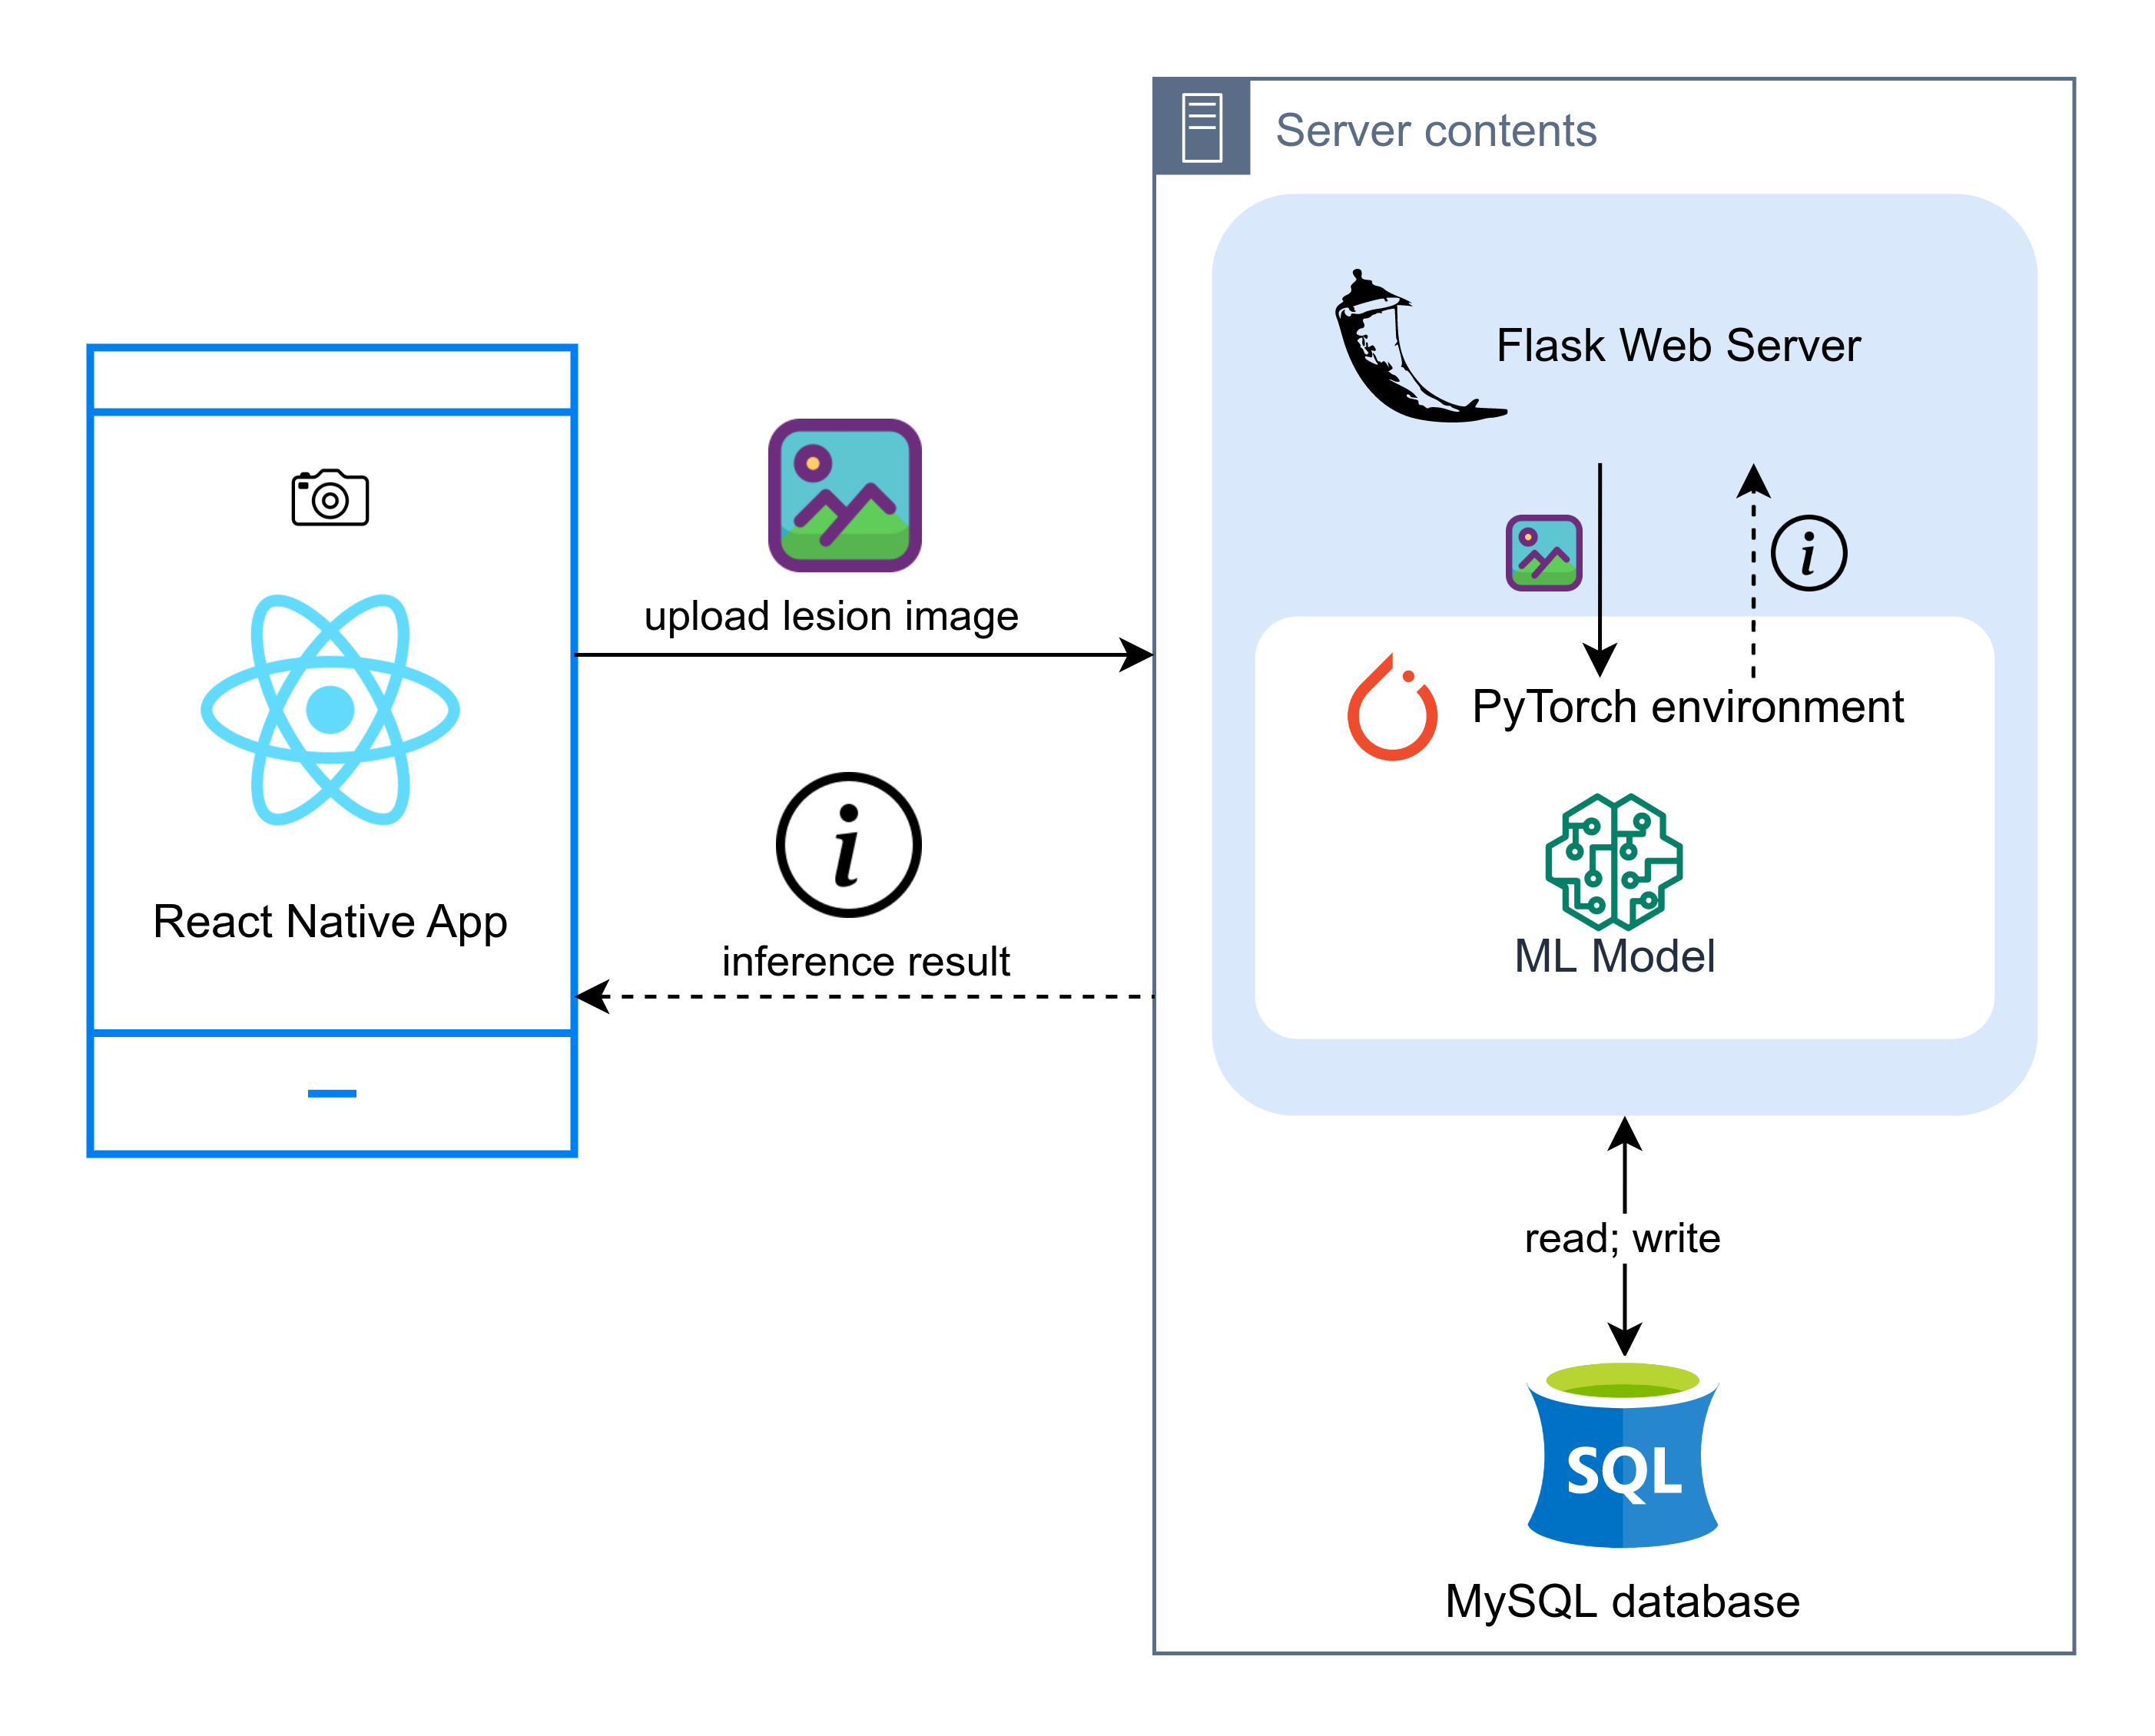
\includegraphics[scale=0.12, fbox]{arch-diagram.png}
    \caption{System architecture diagram}
    \label{fig:arch-diagram}
\end{figure}
\clearpage
\section{System Implementation and Testing}
\subsection{Introduction}
This chapter discusses how the developed solution was implemented and tested. The hardware and software specifications of the implementation environment are discussed, followed by the description of the dataset used. Moreover, the description of training and the description of testing is discussed. The chapter concludes by discussing the testing paradigm used and the testing results.
\subsection{Description of the Implementation Environment}
\subsubsection{Hardware Specifications}
The minimum hardware specifications of the developed solution are as shown in Table \ref{tab:hardware} below. The developed solution is composed of a minimum of two devices interacting which include: a web server and a mobile device.
\renewcommand{\arraystretch}{1.5}
\setlength{\tabcolsep}{18pt}
\begin{xltabular}{1\textwidth} {
        | >{\raggedright\arraybackslash}c
        | >{\raggedright\arraybackslash}X
        | >{\raggedright\arraybackslash}X
        |}
    \hline
    \textbf{Device} &
    \textbf{Hardware} & \textbf{Description and Justification}\\\hline
    \multirow{3}{4em}{Web server} &
    CPU: at least 1 gigahertz clock speed & This is the minimum requirement for installing Ubuntu Server Edition operating system. Moreover, the machine learning model uses the CPU to perform inference.\\\cline{2-3}
    & 2 Gigabytes of RAM & This ensures that the Ubuntu Server OS runs smoothly and can also effectively host a web server capable of performing inference for image classification.\\\hline
    & 4 Gigabytes of disk space & Ubuntu Server Edition OS needs a minimum of 2.5 Gigabytes of disk space and the remaining 1.5 Gigabytes is space for installing software packages, storing web server code and storing image uploads.\\\hline

    \multirow{3}{4em}{Mobile device} &
    CPU: Quad Core 1.3 gigahertz clock speed & Required to run Android 5 OS and higher.\\\cline{2-3}
    & 1 Gigabyte of RAM & This is the minimum requirement to run Android 5 or higher.\\\cline{2-3}
    & 100 Megabytes of disk space & This storage space is required to install the application and to be able to take photos and store them.\\\hline
    \caption{Table showing hardware specifications}
    \label{tab:hardware}
\end{xltabular}

% \end{longtable}
\subsubsection{Software Specifications}
The developed solution is composed of the following software components: a mobile application, and a RESTful API. The software specifications for the above software components are as shown in Table \ref{tab:software} below.
\clearpage
\begin{xltabular}{1\textwidth} {
        | >{\raggedright\arraybackslash}c
        | >{\raggedright\arraybackslash}X
        |}
    \hline
    \textbf{Software} & \textbf{Description and Justification}\\\hline
    Android 5+ and iOS 13+ & Since, the mobile application for the developed solution is built using Expo, which is a React Native framework, the mobile devices need to run Android 5+ and iOS 13+.\\\hline
    Expo SDK 46 & The mobile application was written using Expo SDK 46, hence it is required for one to run the project and build application bundles for distribution on Play Store and App Store. Expo was used because of the convenience of being ab;e to write cross-platform applications in Javascript.\\\hline
    Flask & The RESTful API was written using Flask,  a micro web framework written in Python. Flask was used because of its simplicity and also because the machine learning model could easily be run from the same API.\\\hline
    NPM(Node Package Manager) & Node package manager were used to install, update and manage dependencies for the development of the mobile application.\\\hline
    PIP & PIP was used to install and manage software packages for the development of the RESTful API.\\\hline
    PyTorch & PyTorch was used as the machine learning framework. Its torch and torchvision packages were used.\\\hline
    \caption{Table showing software specifications}
    \label{tab:software}
\end{xltabular}
\subsection{Description of the Dataset}
To train the model used in the developed solution and five different but related datasets were combined and used. The datasets used are shown in Table \ref{tab:datasets2}. The datasets consisted of images of two classes: malignant melanoma and benign nevus. The number of images for each class is shown in Table \ref{tab:class_img_count} below. All the datasets were downloaded from where they were hosted on the internet with all of them being used and cited in published research.
\begin{table}[h]
    \centering
    \begin{tabular}{|l|l|l|}
        \hline
        \textbf{Dataset}                     & \textbf{Publisher}       & \textbf{No. of images} \\\hline
        MED-NODE                             & \cite{giotis2015med}     & 170                    \\\hline
        PAD-UFES-20                          & \cite{PACHECO2020103545} & 296                    \\\hline
        7-point                              & \cite{8333693}           & 827                    \\\hline
        DermIS                               & \cite{dermis}            & 69                     \\\hline
        DermQuest                            & Galderma S.A.            & 137                    \\\hline
        \multicolumn{2}{|r|}{\textbf{Tota}l} & \textbf{1499}                                     \\\hline
    \end{tabular}
    \caption{Table showing list of datasets to be used}
    \label{tab:datasets2}
\end{table}

Before the ensemble dataset could be used, it had to be pre-processed. Using the metadata accompanying the datasets, Talend, an ETL tool, was used to combine the datasets into a uniform and orderly whole. The PAD-UFES-20 dataset~\citep{PACHECO2020103545} and the 7-point dataset~\citep{8333693} included images for other types of skin cancer which were not used to train the model. Hence, Talend was used to extract the images corresponding to malignant melanoma and benign naevi from those datasets.

\begin{table}[h]
    \centering
    \begin{tabular}{|c|c|c|}
        \hline
        \textbf{Class}      & \textbf{Count} & \textbf{Percentage} \\\hline
        Malignant Melanoma  & 493            & 32.89\%             \\\hline
        Benign Nevus(naevi) & 1006           & 67.11\%             \\\hline
    \end{tabular}
    \caption{Table showing number of images for each class}
    \label{tab:class_img_count}
\end{table}

The combined dataset was split into train, test and validation subsets as shown in Table \ref{tab:dataset-split} below. Since the five datasets were drawn from slightly different distributions and owing to the class imbalance as can be seen in Table \ref{tab:class_img_count}, random stratified sampling was used to split the combined dataset such that all the different distributions and the two classes were represented proportionately in the train, validation and evaluation sets.

\begin{table}[h]
    \centering
    \begin{tabular}{|c|c|}
        \hline
        \textbf{Subset} & \textbf{Percentage} \\\hline
        Train Set       & 70\%                \\\hline
        Validation Set  & 15\%                \\\hline
        Evaluation Set  & 15\%                \\\hline
    \end{tabular}
    \caption{Table showing training, validation and evaluation sets split}
    \label{tab:dataset-split}
\end{table}

Figure \ref{fig:samples} below shows a sample of images from the ensemble dataset where the images labelled `melanoma' correspond to malignant skin lesions while those labelled `nevus' correspond to benign skin lesions.

\begin{figure}[h]
    \centering
    \setlength{\fboxsep}{8pt}
    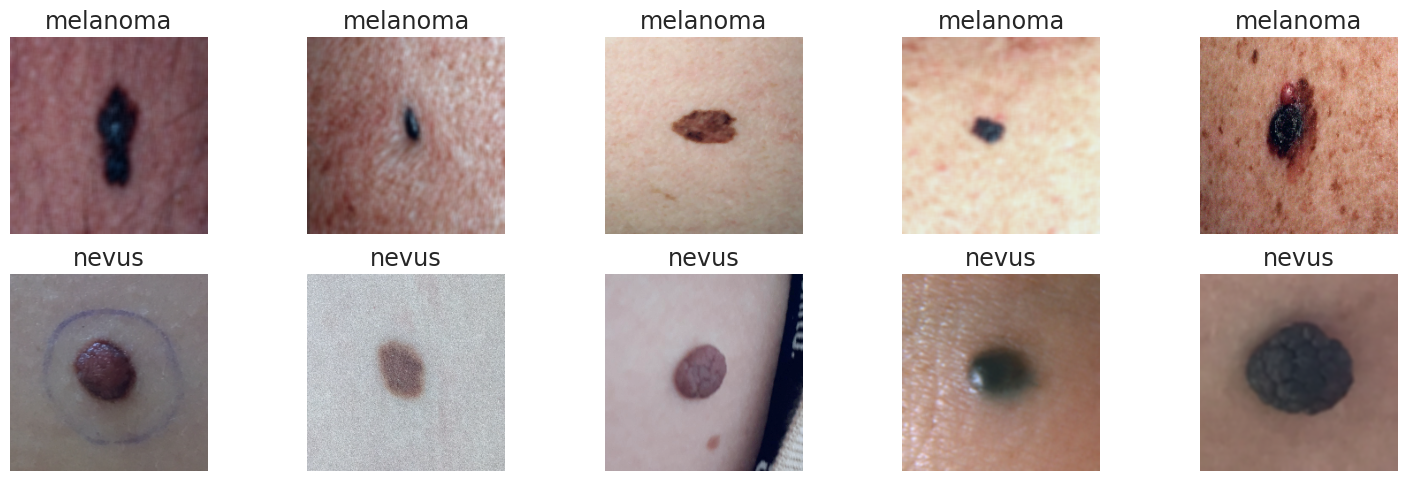
\includegraphics[scale=0.4, fbox]{images/samples.png}
    \caption{Figure showing sample images from the ensemble dataset}
    \label{fig:samples}
\end{figure}


\subsection{Description of Training}
This section discusses how the segmentation and classification models were trained and various experiments conducted during model training which include: exploring learning rate schedulers, investigating the effect of data augmentation on performance, investigating the effect of image segmentation on performance and exploring transfer learning with different pre-trained models. All training experiments were done using Pytorch and hosted on Google Colaboratory. In order to ensure the reproducibility of the experiments, random number generators in the execution environment were seeded.

\subsubsection{Training of Classification Models}
The loss function used to train classification models was the Cross-Entropy Loss function whose equation is shown below, where $log$ is natural logarithm, $p_{o,c}$ is the predicted probability for a class $c$, $y_{o,c}$ is the binary target label for a class $c$ and $M$ is the number of classes which in this case is $2$.

\begin{equation}
    -\sum_{c=1}^My_{o,c}\log(p_{o,c})
\end{equation}
\label{eq:5.1}
\myequations{Cross-Entropy loss funtion}

The optimizer used was Adam which in full form is Adaptive Moment Estimation. An early stopping technique was used to prevent overfitting of the model and reduce training time. All models used were initialized with pre-trained weights. Only the classification layers of the neural network models were replaced in order to carry out binary classification as opposed to multiclass classification which they were trained on using the Imagenet dataset. For this reason, the models' classifier parameters were fine-tuned for several epochs while freezing the rest of the network parameters to ensure the stability of the model.

Before feeding images to the models, images were read from storage to memory and resized to $256 * 256$ pixels, centre-cropped to $224 * 224$, standardised using mean and standard deviation values for the red, green and blue channels shown in Table \ref{tab:mean-std-values} below and finally converted into Pytorch tensors. Checkpoints used were selected based on the loss evaluated on the validation set where checkpoints with the least loss for each of the pre-trained models were chosen.

\begin{table}[h]
    \centering
    \begin{tabular}{|l|l|l|}
        \hline
        \textbf{Channel} & \textbf{Mean} & \textbf{Standard deviation} \\\hline
        Red              & 0.485         & 0.229                       \\\hline
        Green            & 0.456         & 0.224                       \\\hline
        Blue             & 0.406         & 0.224                       \\\hline
    \end{tabular}
    \caption{Table showing image standardization values for RGB channels}
    \label{tab:mean-std-values}
\end{table}

\subsubsection{Training U-Net Segmentation Model}
According to the study conducted by \cite{codella2017deep}, image segmentation leads to better performance in the classification of melanoma skin lesions. This study was the basis of the incorporation of image segmentation during model training. The image segmentation model used was U-Net which was implemented and trained using the Dermis and DermQuest datasets which included lesion images and ground truth segmentation masks. The two datasets were combined and splits into train and validation sets comprising 80\% and 20\% of the total number of images respectively. In order to improve segmentation performance and reduce overfitting data augmentation was applied comprising of probabilistic transformations of rotation, horizontal flip and vertical flip.

The loss function used was the Cross-Entropy Loss function depicted in Equation 5.1. Before feeding images to the model images were read from storage to memory and resized to $350 * 350$ pixels, standardised using a mean of 0 and standard deviation of 1 for the red, green and blue channels and finally converted into Pytorch tensors.

\subsubsection{Exploring Learning Rate Schedulers}
Various learning rate schedulers were used including Cosine Annealing with Warm Restarts, One Cycle learning rate scheduler and the Step Learning rate scheduler. Upon training and evaluation, the One Cycle learning rate scheduler was chosen since it had the best evaluation metrics performance as shown in Table \ref{tab:lr-schedulers} below (highest scores per metric are in bold).

\begin{xltabular}{1\textwidth} {
        | >{\raggedright\arraybackslash}X
        | >{\raggedright\arraybackslash}X
        | >{\raggedright\arraybackslash}X
        | >{\raggedright\arraybackslash}X
        | >{\raggedright\arraybackslash}X
        |}
    \hline
    \textbf{Learning rate scheduler} & \textbf{Accuracy} & \textbf{F1-Measure} & \textbf{Sensitivity} & \textbf{Specificity}\\\hline
    Cosine Annealing with Warm Restarts & 0.7753 & 0.7753 & 0.8410 & 0.64473\\\hline
    One Cycle & \textbf{0.8326} & \textbf{0.8716} & 0.8543 & \textbf{0.7894}\\\hline
    Step & 0.8061 & 0.8061 & \textbf{0.9006} & 0.6184\\\hline
    \caption{Table showing testing results for various learning rate schedulers}
    \label{tab:lr-schedulers}
\end{xltabular}

\subsubsection{Effect of Data Augmentation}
According to \cite{perez2021convolutional}, data augmentation is a technique of expanding the size of a dataset by applying several random transformations to original images. The Albumenation library developed by \cite{buslaev2020albumentations} was used where a series of transformations were applied to the images with a given probability of being applied. Applying these transformations had the effect of increasing the number of samples in the dataset without actually saving new images to storage since the transformations are applied with a given probability, hence different images with different transformations were fed to the model across the epochs. The transformation applied and listed in Table \ref{tab:augmentations} below.
\begin{xltabular}{1\textwidth} {
        | >{\raggedright\arraybackslash}X
        | >{\raggedright\arraybackslash}X
        | >{\raggedright\arraybackslash}X
        |}
    \hline
    \textbf{Transformation} & Description & Probability \\\hline
    Random rotate 90 degrees & Randomly rotate the input by 90 degrees zero or more times. & 0.5\\\hline
    Flip & Flip the input either horizontally, vertically or both. & 0.5\\\hline
    Transpose & Transpose the input by swapping rows and columns. & 0.5\\\hline
    Additive Gaussian Noise & Add Gaussian noise & 0.5\\\hline
    Blur & Blur the input image using a random-sized kernel. & 0.05\\\hline
    Motion blur & Apply motion blur to the input image. & 0.1\\\hline
    Median blur & Blur the input image using a median filter & 0.05\\\hline
    Random brightness and contrast & Randomly change the brightness and contrast of the input image. & 0.3\\\hline
    Hue, saturation and value & Randomly change the hue, saturation and value of the input image. & 0.3\\\hline
    Gaussian Blur & Blur the input image using a Gaussian filter with a random kernel size. & 0.5\\\hline
    \caption{Table listing data augmentation transformations}
    \label{tab:augmentations}
\end{xltabular}

The use of data augmentation led to significantly better performance as compared to training without data augmentation as shown in Table \ref{tab:augmentation-results} using the Resnet34 model. The increase in performance as a result of data augmentation can be explained by Figure \ref{fig:resnet34_aug} which depicts the graphs of validation loss against epochs and accuracy against epochs. The trend of the curves suggests more resistance to overfitting compared to the same graphs for training without data augmentation shown in Figure \ref{fig:resnet34_no_aug} (highest scores per metric are in bold).

\begin{figure}[h]
    \centering
    \setlength{\fboxsep}{8pt}
    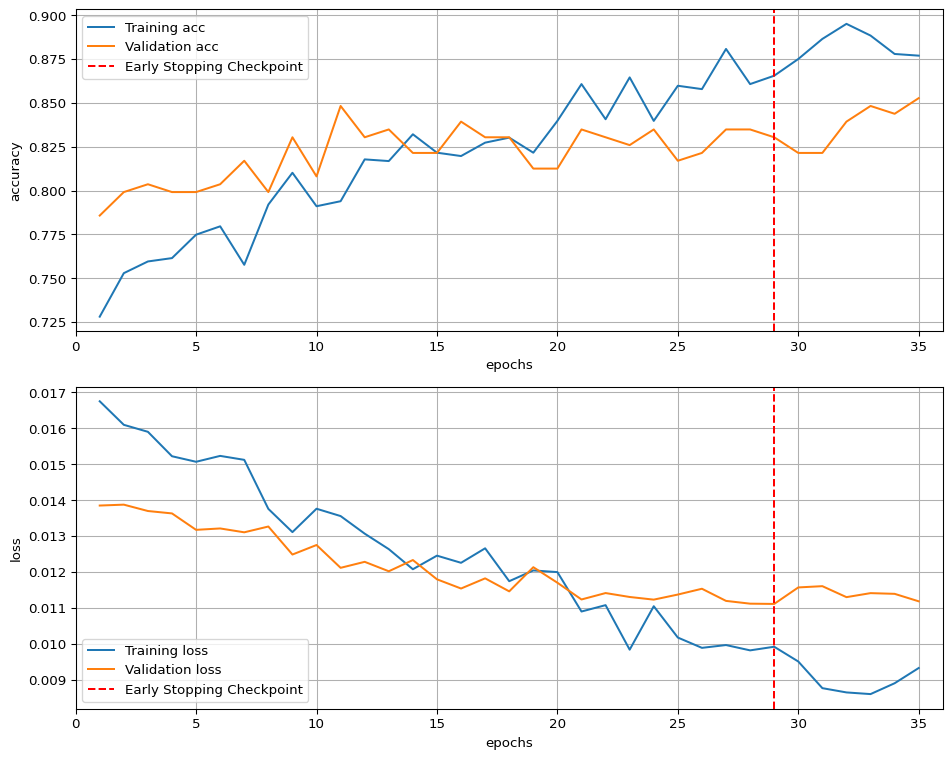
\includegraphics[scale=0.5, fbox]{images/resnet34-aug-loss.png}
    \caption{Graphs of loss and accuracy against epochs(using data augmentation)}
    \label{fig:resnet34_aug}
\end{figure}

\begin{figure}[h]
    \centering
    \setlength{\fboxsep}{8pt}
    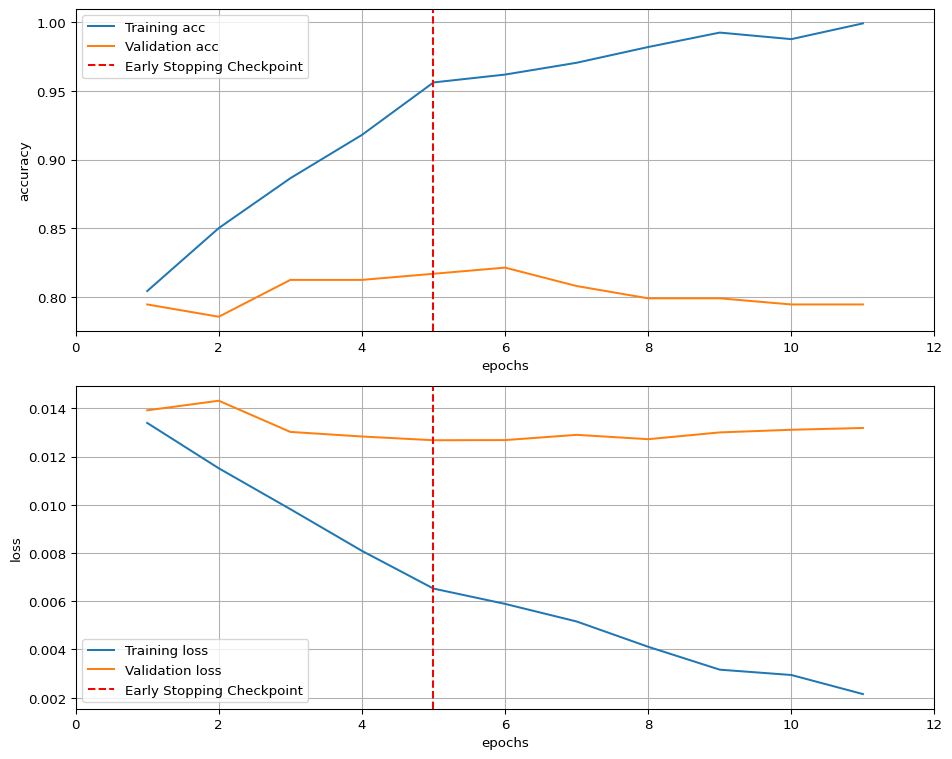
\includegraphics[scale=0.5, fbox]{images/resnet34-noaug-loss.png}
    \caption{Graphs of loss and accuracy against epochs(without data augmentation)}
    \label{fig:resnet34_no_aug}
\end{figure}


\begin{xltabular}{1\textwidth} {
        | >{\raggedright\arraybackslash}X
        | >{\raggedright\arraybackslash}X
        | >{\raggedright\arraybackslash}X
        | >{\raggedright\arraybackslash}X
        | >{\raggedright\arraybackslash}X
        |}
    \hline
    & \textbf{Accuracy} & \textbf{F1-Measure} & \textbf{Sensitivity} & \textbf{Specificity}\\\hline
    Without augmentation & 0.7929 & 0.7929 & \textbf{0.8741} & 0.6316\\\hline
    With augmentation & \textbf{0.8326} & \textbf{0.8716} & 0.8543 & \textbf{0.7894}\\\hline
    \caption{Table showing testing results of data augmentation experiments}
    \label{tab:augmentation-results}
\end{xltabular}

\subsubsection{Effect of Image Segmentation}
Using a pre-trained ResNet34 model, performance was compared when training the model using segmented lesion images and non-segmented lesion images. As shown in Table \ref{tab:segementation} below, segmentation led to a poorer performance as compared to training without image segmentation across all evaluation metrics (highest scores per metric are in bold). As a result, the developed solution does not include image segmentation. These results affirm the findings of \cite{7493528}, who asserts that image segmentation is a non-trivial task which risks leaving out important features hence negatively impacting classification performance.

\begin{xltabular}{1\textwidth} {
        | >{\raggedright\arraybackslash}X
        | >{\raggedright\arraybackslash}X
        | >{\raggedright\arraybackslash}X
        | >{\raggedright\arraybackslash}X
        | >{\raggedright\arraybackslash}X
        |}
    \hline
    & \textbf{Accuracy} & \textbf{F1-Measure} & \textbf{Sensitivity} & \textbf{Specificity}\\\hline
    With segmentation & 0.7577 & 0.7577 & 0.8476 & 0.5789\\\hline
    Without segmentation & \textbf{0.8326} & \textbf{0.8716} & \textbf{0.8543} & \textbf{0.7894}\\\hline
    \caption{Table showing testing results of image segmentation experiments}
    \label{tab:segementation}
\end{xltabular}

\subsubsection{Transfer Learning with Different Pretrained Models}
Research has shown that transfer learning significantly increases model accuracy while reducing training time and computing resources. The pre-trained models used included ResNet34, ResNet50, ResNet152, InceptionV3, EfficientNetV2 and VisionTransformer. All of the models were initialized with  pre-trained weights trained on Imagenet~\citep{deng2009imagenet} which is a large-scale hierarchical image database commonly used as a computer vision benchmark dataset. The performance metrics of the trained models are discussed in Section 5.5.
\subsection{Description of Testing and Evaluation}
In order to test and evaluate the models trained the validation set and evaluation set respectively (listed in Table \ref{tab:dataset-split}), were used.
\subsubsection{Evaluation Metrics Used}
Evaluation metrics used include accuracy, sensitivity, specificity, F1-measure, and dice score which are expounded on in Table \ref{tab:metrics} below.

\begin{xltabular}{1\textwidth} {
        | >{\raggedright\arraybackslash}l
        | >{\raggedright\arraybackslash}X
        | >{\raggedright\arraybackslash}c
        | }
    \hline
    \textbf{Metric} & \textbf{Description} & \textbf{Equation}\\\hline
    Sensitivity & Measures model's ability to predict true positives as positive. &
    \begin{equation}
        = \frac{TP}{TP+FN}
    \end{equation}
    \label{eq:5.2}
    \myequations{Equation for sensitivity}
    \\\hline
    Specificity & Measures model's ability to predict true negatives as negative &
    \begin{equation}
        \frac{TN}{FP+TN}
    \end{equation}
    \label{eq:5.3}
    \myequations{Equation for specificity}
    \\\hline
    F1-Measure & Harmonic mean of precision and recall &
    \begin{equation}
        = \frac{2*TP}{2*TP+FP+FN}
    \end{equation}
    \label{eq:5.4}
    \myequations{Equation for F1-Measure}
    \\\hline
    Accuracy & Ratio of total correctly classified observation to the total number of observations &
    \begin{equation}
        = \frac{TP+TN}{TP+TN+FP+FN}
    \end{equation}
    \label{eq:5.5}
    \myequations{Equation for accuracy}
    \\\hline
    Dice Score & Is a metric used to gauge image segmentation performance which is the ratio between twice the area of overlap between the region of an image and its segmentation mask, to the total number of pixels in an image and its segmentation mask &
    \begin{equation}
        = \frac{2 |U \cap V| }{ |U \cup V| }
    \end{equation}
    \label{eq:5.6}
    \myequations{Equation for dice score}
    \\\hline
    % AUROC Score & Area under true positive ratio against false positive ratio & Area under ROC curve\\\hline
    \caption{Table showing evaluation metrics used}
    \label{tab:metrics}
\end{xltabular}


\subsubsection{Experimental Results}
The U-Net model was trained to segment skin lesions using the DermIS and DermQuest datasets which had ground truth image segmentation marks. The U-Net model obtained an accuracy of 0.9232 and a dice score of 0.7414 on its validation set.

Table \ref{tab:exp-results} show the performance metrics of the classification models resulting from training (the highest scores per metric are in bold). The models were trained using the one-cycle learning rate scheduler, with data augmentation applied and without image segmentation.
\begin{xltabular}{1\textwidth} {
        | >{\raggedright\arraybackslash}X
        | >{\raggedright\arraybackslash}X
        | >{\raggedright\arraybackslash}X
        | >{\raggedright\arraybackslash}X
        | >{\raggedright\arraybackslash}X
        | >{\raggedright\arraybackslash}X
        |}
    \hline
    \textbf{Model} & \textbf{Accuracy} & \textbf{F1-Measure} & \textbf{Sensitivity} & \textbf{Specificity} & \textbf{Average}\\\hline
    Resnet34 & \textbf{0.8326} & 0.8716 & 0.8543 & 0.7894 & \textbf{0.8370}\\\hline
    Resnet50 & 0.7974 & 0.8392 & 0.7947 & \textbf{0.8026} & 0.8085\\\hline
    Resnet152 & \textbf{0.8326} & 0.8701 & 0.8874 & 0.6974 & 0.8197\\\hline
    InceptionV3 & 0.8194 & 0.8707 & \textbf{0.9139} &  0.6316 & 0.8089\\\hline
    EfficientNetV2 & 0.8194 & 0.8638 & 0.8609 & 0.7368 & 0.8202\\\hline
    VisionTransformer & 0.8282 & \textbf{0.8762} & 0.9139 & 0.6579 & 0.8190\\\hline
    \caption{Table showing testing results for various pre-trained models}
    \label{tab:exp-results}
\end{xltabular}

Confusion matrices for the Resnet34, Resnet50, Resnet152, InceptionV3, EfficientNetV2 and VisionTransfomer are displayed in Appendix I. From the experimental results, it turned out that the best model is Resnet34 since it has the highest average score which was calculated as the arithmetic mean of accuracy, precision, sensitivity and specificity. For this reason, the trained Resnet34 was used for classification in the developed solution.

\subsection{Testing Paradigm}
A hybrid test paradigm was used for the developed solution comprising black box testing, white box testing and unit testing.

\subsubsection{Black Box Testing}
Black box testing is a software validation technique where the correctness and appropriateness of software are evaluated based on its output in response to an input given and conditions it is subjected to without investigating the internal workings of the software being tested~\cite{nidhra2012black}. Black box comprised the majority of the test coverage and it was used to validate the functioning of the RESTful API and the mobile application.
\subsubsection{White Box Testing}
White box testing is a software validation technique where the internal workings of implementation source code are investigated to identify bugs in software~\cite{nidhra2012black}. white box testing was used throughout the development process to ensure that the source code actually did what it was intended to do. White box testing to ensure the correctness of the source code for the RESTful API and the mobile application.
% \subsubsection{Unit Testing}
% Unit testing is a software validation technique that involves the testing of a unit of code such as a function or anything no more than a class, where actual results of the executed unit of code are compared with the expected results~\citep{olan2003unit, nidhra2012black}. Unit testing was used to test functions used during the training of the model. The various routes of the RESTful API were also tested using unit testing. Key functions in the mobile app source code were also tested using unit testing.
\subsection{Testing Results}
Table \ref{tab:testing-results-api} shows the results of black box testing carried out on the Flask RESTful API.

\renewcommand{\arraystretch}{1.0}
\setlength{\tabcolsep}{6pt}
\begin{xltabular}{1\textwidth} {
        | >{\raggedright\arraybackslash}X
        | >{\raggedright\arraybackslash}X
        | >{\raggedright\arraybackslash}X
        | >{\raggedright\arraybackslash}X
        | >{\raggedright\arraybackslash}X
        |}
    \hline
    \textbf{Test Case} & \textbf{Description} & \textbf{Test Data} & \textbf{Result} & \textbf{Test Verdict}\\\hline
    TC01: Obtaining prediction for a lesion image & Attempt made to upload image to API, get inference and store record in database & POST HTTP request to http://<ip address>:port/api/lesions/<id>, where <id> is the user's id & Inference result returned for image and new record created for it. & Pass\\\hline
    TC02: Retrieving list of past predictions & Attempt made to retrieve list of past predictions for a given user & GET HTTP request to http://<ip address>:port/api/lesions/<id>, where <id> is the user id of the currently logged in user. & JSON array of existing predictions in the lesion table is returned. & Pass\\\hline
    TC03: Deleting past prediction & Attempt made to delete past prediction from database. & DELETE HTTP request to http://<ip address>:port/api/lesions/<id>, where <id> is an id for a well-known past prediction & Message for successful deletion returned and recorded deleted from lesions table & Pass\\\hline

    \caption{Table showing testing results for the RESTful API}
    \label{tab:testing-results-api}
\end{xltabular}

Table \ref{tab:testing-results-app} below shows the results of the testing carried out on the developed mobile app.

\renewcommand{\arraystretch}{1.0}
\setlength{\tabcolsep}{6pt}
\begin{xltabular}{1\textwidth} {
        | >{\raggedright\arraybackslash}X
        | >{\raggedright\arraybackslash}X
        | >{\raggedright\arraybackslash}X
        | >{\raggedright\arraybackslash}X
        | >{\raggedright\arraybackslash}X
        |}
    \hline
    \textbf{Test Case} & \textbf{Description} & \textbf{Test Data} & \textbf{Result} & \textbf{Test Verdict}\\\hline
    TC04: Taking lesion photo & Attempt made to take a photo of skin lesion & Tap button with camera icon then take photo & User is redirected to the camera app and photo taken and saved to device storage and displayed to user in the app. & Pass\\\hline
    TC05: Selecting lesion photo & Attempt made to select existing lesion photo from storage & Tapping the "Select image" button & User is directed to a file picker allowing picking of images only and selected image displayed in the app. & Pass\\\hline
    TC06: Uploading lesion photo for inference & Attempt made to upload and obtain inference for a lesion photo & Tap camera icon button, then take lesion photo, tap the check icon and wait & User is directed to camera app, takes photo, photo is successfully uploaded and inference results displayed. & Pass\\\hline
    TC07: Viewing past predictions & Attempt made to obtain a prediction and confirm its presence in history of past predictions & Tap camera icon button, take a photo, upload photo and get prediction. Then press back and click on history icon button & After obtaining prediction, a record of the new prediction was seen to appear under the list of past predictions. & Pass\\\hline
    TC08: Deleting past prediction & Attempt made to delete past prediction entry & Tap history icon and press delete bin icon of an entry & On pressing the delete bin icon for an entry, the entry is removed from list of past predictions. & Pass\\\hline

    \caption{Table showing testing results for the mobile application}
    \label{tab:testing-results-app}
\end{xltabular}

\clearpage
\section{Conclusions, Recommendations and Future Works}
\subsection{Conclusions}
Having obtained high-performance metric scores for the Resnet34 model (accuracy of 0.8326, F1-Measure of 0.8716, sensitivity of 0.8543 and specificity of 0.7894) for the classification of melanoma skin lesions, it can be concluded that indeed the developed solution can reliably be used to support the diagnosis of melanoma where there are few diagnostic specialists and increase chances of early detection of melanoma. Furthermore, this study showed that the segmentation of skin lesion images before classification negatively impacts classification performance. Additionally, it was concluded that data augmentation significantly increases model performance by reducing overfitting.
\subsection{Recommendations}
It is recommended that for training various deep learning models, the reproducibility of the results should be taken into account in order to ensure consistent results and conclusions. This is because the training of deep learning models involves the use of random number generators hence if random number generators are not seeded inconsistent results will be obtained.
\subsection{Future Works}
In view of the limitation on the size of melanoma skin lesion datasets, future works in this area should focus on the collection of more non-dermoscopic images to create larger datasets in order to increase confidence in the performance of deep learning models.
\clearpage
\bibliography{bibliography}
\bibliographystyle{apalike}
\clearpage
\section*{Appendices}
\addcontentsline{toc}{section}{Appendices}
\captionsetup[figure]{list=no}
\subsection*{Appendix I: Confusion Matrices for Trained Models}
\addcontentsline{toc}{subsection}{Appendix I: Confusion Matrices for Trained Models}
\begin{figure}[h]
    \centering
    \setlength{\fboxsep}{8pt}
    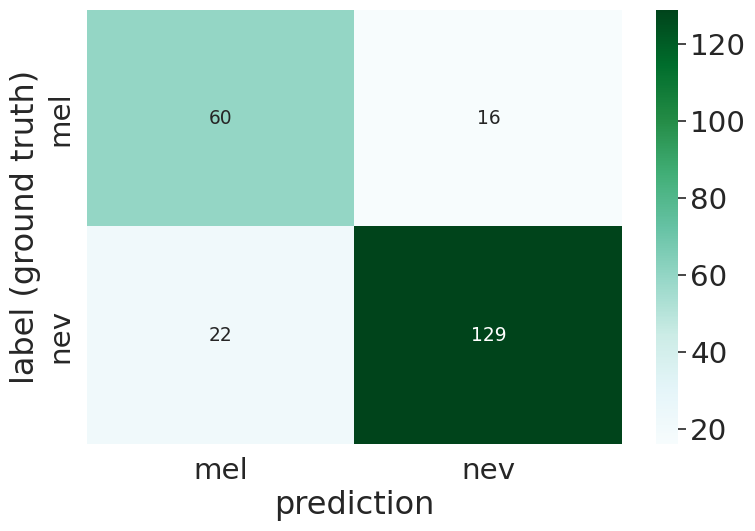
\includegraphics[scale=0.5, fbox]{images/matrix-resnet34.png}
    \caption{Confusion matrix for Resnet34}
    \label{fig:matrix-resnet34}
\end{figure}

\begin{figure}[h]
    \centering
    \setlength{\fboxsep}{8pt}
    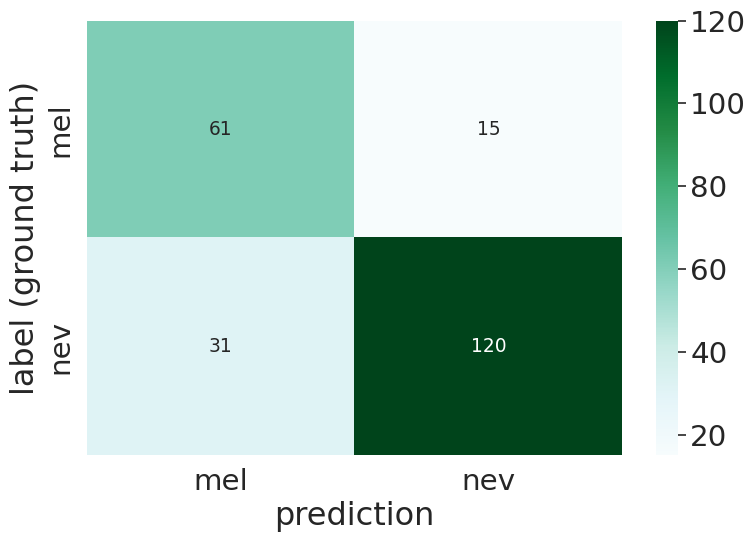
\includegraphics[scale=0.5, fbox]{images/matrix-resnet50.png}
    \caption{Confusion matrix for Resnet50}
    \label{fig:matrix-resnet50}
\end{figure}

\begin{figure}[h]
    \centering
    \setlength{\fboxsep}{8pt}
    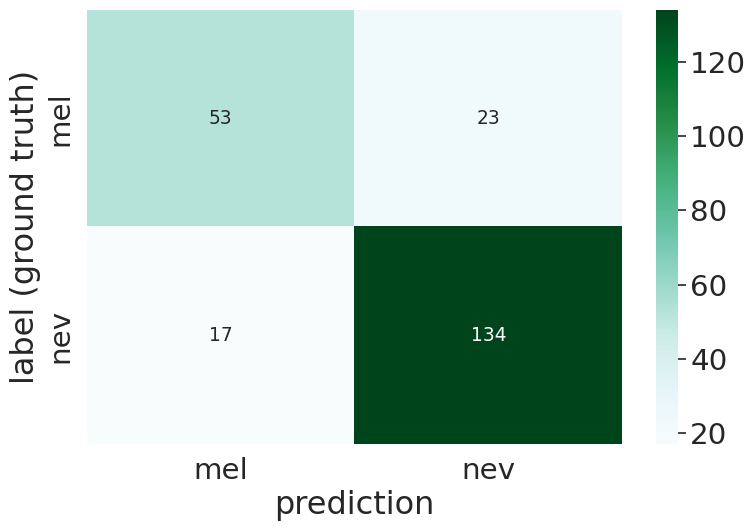
\includegraphics[scale=0.5, fbox]{images/matrix-resnet152.png}
    \caption{Confusion matrix for Resnet152}
    \label{fig:matrix-resnet152}
\end{figure}

\begin{figure}[h]
    \centering
    \setlength{\fboxsep}{8pt}
    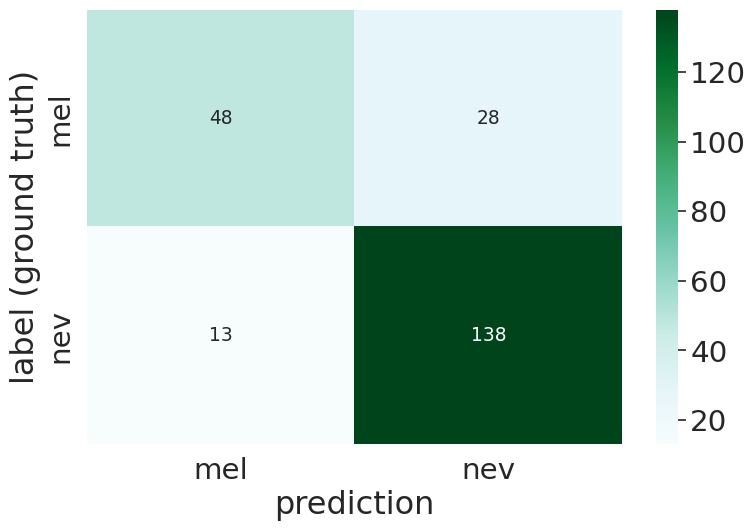
\includegraphics[scale=0.5, fbox]{images/matrix-inceptionv3.png}
    \caption{Confusion matrix for InceptionV3}
    \label{fig:matrix-inceptionv3}
\end{figure}

\begin{figure}[h]
    \centering
    \setlength{\fboxsep}{8pt}
    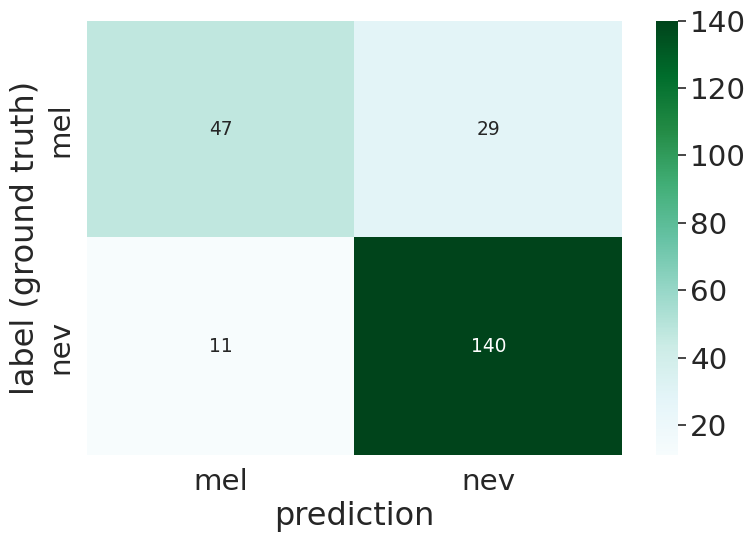
\includegraphics[scale=0.5, fbox]{images/matrix-efficientnet.png}
    \caption{Confusion matrix for EfficientNetV2}
    \label{fig:matrix-efficientnet}
\end{figure}

\begin{figure}[h]
    \centering
    \setlength{\fboxsep}{8pt}
    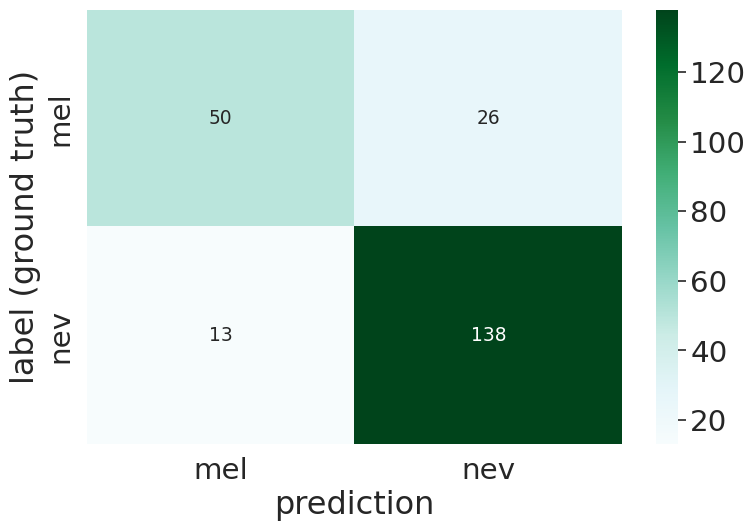
\includegraphics[scale=0.5, fbox]{images/matrix-vit.png}
    \caption{Confusion matrix for VisionTransformer}
    \label{fig:matrix-vit}
\end{figure}
\clearpage
\begin{landscape}
    \thispagestyle{empty}
    \subsection*{Appendix II: Gantt Chart}
    \addcontentsline{toc}{subsection}{Appendix II: Gantt Chart}
    \begin{figure}[h]
        \centering
        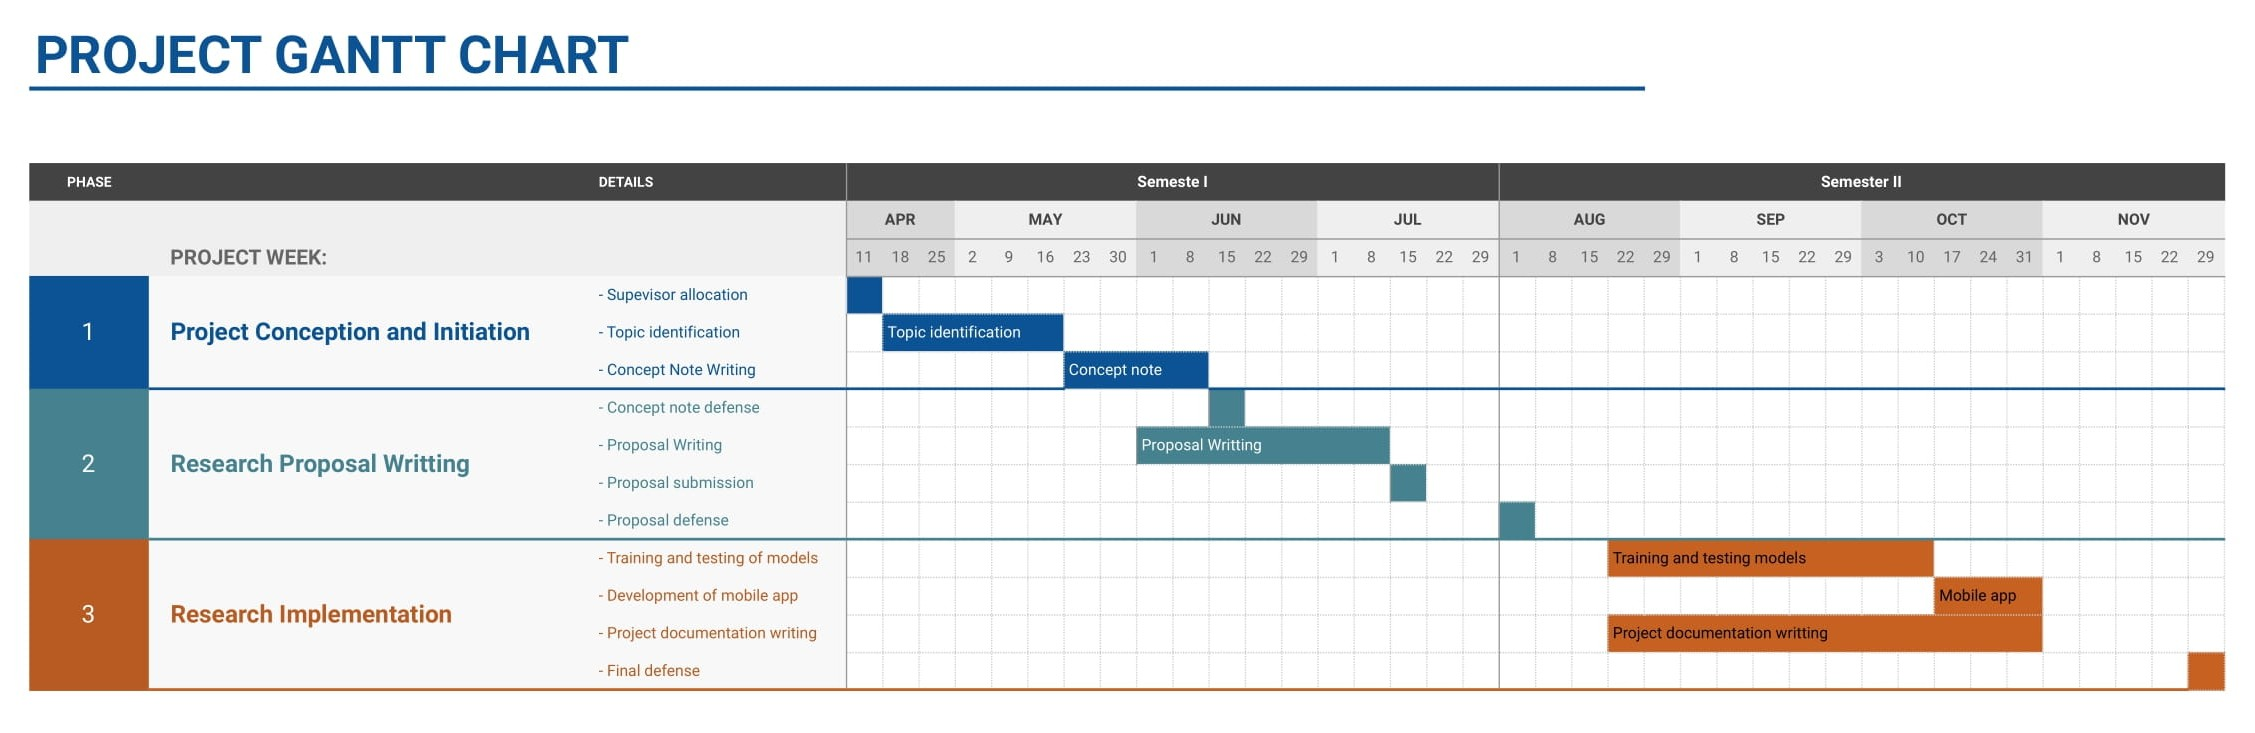
\includegraphics[scale=0.34]{gantt.jpg}
        \caption*{Appendix I: Gantt chart showing project timeline}
    \end{figure}
    \vfill
    \raisebox{0pt}{\makebox[\linewidth]{\thepage}}
\end{landscape}
\end{document}